
	\section{El problema de la distribución espacial del ingreso}
	
El estudio del ingreso ha sido un tema muy caro a las ciencias sociales y sus diversas disciplinas. Constituye un objeto de estudio interesante para la economía en la medida en la medida en que atañe a la tensión entre crecimiento de la economía y asignación de los recursos. El fenómeno de la distribución del ingreso, entendido como nexo entre el desempeño de una economía y las condiciones de vida de la población, adquiere relevancia en dos sentidos: por un lado, al influir sobre la trayectoria de crecimiento de una economía y, por el otro, al dar cuenta de los niveles de desigualdad existentes entre los hogares y personas de una población \cite{giayetto}. 

Además de preguntarse sobre los impactos de una determinada distribución del ingreso en el proceso de crecimiento y desarrollo, desde otros campos disciplinares, la sociología y la ciencia política han procurado en sus desarrollos dar cuenta sobre las implicancias sociales de la distribución del ingreso en términos de estabilidad del orden social y el conflicto político concomitante. Incluso, se ha procurado desde el corpus teórico de las ciencias sociales, ofrecer elementos para del debate en torno a lo que se considera una distribución del ingreso justa y equitativa.   

De este modo, queda explicitado el recorte del objeto de estudio en función de una “relación de valor” \cite{weber},  entendida como aquello que motiva al investigador a delimitar el campo de estudio dentro de la infinitud de datos empíricos, en virtud de la centralidad que tiene este debate más allá de las ciencias sociales. Todo actor social forma “juicios de valor” \cite{weber} sobre una distribución del ingreso "justa". Esta cuestión normativa o ética impacta en las relaciones de valor que se establecen en el método científico a la hora de delimitar objetos de estudio, tal como sostiene Weber. Este punto también es central para autores como David Harvey \citeyear{harvey} que escribe con el intento de suturar el divorcio entre ciencia y postulados normativos. Al mismo tiempo, los planteos de Harvey son de especial interés para este trabajo en la medida en que ofrecen numerosos elementos a la hora de pensar la distribución del ingreso con una dimensión que ha sido soslayada en la teoría: la dimensión espacial. 

Los análisis de la distribución del ingreso en las ciencias sociales han puesto el foco principalmente en la distribución funcional y la distribución personal (la primera poniendo el foco en el retorno a los factores productivos y la segunda en el ingreso individual de cada actor, amen a qué factor productivo pertenezca). Sin embargo, existe otra clave de análisis: la espacial o geográfica. La misma enfoca la cuestión analizando la comparación de diferentes áreas geográficas en términos de su ingreso \cite{gasparini2001}. Este análisis puede combinarse con los análisis funcionales, atendiendo a los factores productivos y su ubicación geográfica, o puede realizarse un análisis de la distribución del ingreso personal en diferentes zonas geográficas. Se han desarrollado investigaciones en torno a la distribución del ingreso entre países, ya sea tomando el ingreso total basándose en sus cuentas nacionales y calculándolo en base al PBI \cite{theil} o en base a distribuciones del ingreso personal utilizando encuestas de ingresos y gastos \cite{milanovic2002,milanovic2005,davies}. También se han realizado entre regiones o provincias de un país \cite{artana} que pueden hacer referencia al ingreso total utilizando como base el producto bruto geográfico (PBG) \cite{altimir1975}.

A su vez, y es el camino que se emprenderá en este trabajo, es plausible analizar la distribución del ingreso hacia el interior de un aglomerado urbano \cite{gasparini2000,giayetto}. De hecho, se planteará que el interés de abordar la temática desde la perspectiva espacial no se limita a describir cómo el ingreso se distribuye de modo independiente y azaroso en el espacio, tomando una mera distribución espacial en un espacio de coordenadas bidimensional. Los aportes de la sociología urbana han sido precisamente los de buscar establecer cómo el espacio urbano socialmente producido guarda una relación con la distribución del ingreso que \textit{tiene lugar} en dicho espacio (ya sea entre las personas o entre los factores que allí se \textit{localizan}). La diferencia entre las corrientes de la sociología urbana se dan en función de la naturaleza de esa relación: mientras que para la escuela ecologista de Chicago \cite{park,burgess1928,mckenzie,wirth} se podría sostener que se trata de una relación unidireccional donde las determinaciones del espacio priman, para la escuela crítica \cite{lefebvre,castells,harvey} la misma es de naturaleza dialéctica y por lo tanto, el espacio condiciona los procesos sociales, pero a su vez se puede dar cuenta de una producción social del espacio urbano. Estas diferencias se verán con mayor detalle al recorrer los antecedentes teóricos de los que este trabajo se nutre.


Desde el punto de vista metodológico, tema que será abordado con mayor detalle en le próximo capítulo, cada dimensión del ingreso tiene su correspondiente set de instrumentos metodológicos para la medición de su distribución. Por un lado, la distribución funcional, las cuentas nacionales proveen la información suficiente para establecer qué parte del ingreso, como contracara del producto, es retribución del factor trabajo, capital o tierra \cite{grania}. Existen, para esta medición, dificultades intrínsecas a la hora de abordar los impuestos como así también situaciones que tienen que ver con los cambios en el mundo laboral reciente, pero que exceden los objetivos de este trabajo. Por otro lado, los análisis de la distribución personal del ingreso han producido numerosas metodologías para su medición entre las cuales se encuentran los conocidos índices de Gini, Atkinson, Theil entre otros \cite{worldbank}, que toman como principal fuente las encuestas nacionales o registros administrativos sobre trabajo e ingresos.

Mas a la hora de analizar la distribución personal del ingreso en su dimensión geográfica o espacial, existe otro desafío. Las mencionadas encuestas nacionales y provinciales de empleo que miden ingresos no ofrecen un nivel de desagregación geográfica suficiente para hacerlo en áreas geográficas pequeñas. Las muestras que las componen ofrecen un nivel de representatividad para grandes aglomerados, por lo cual pueden obtenerse estadísticos de interés con suficiente representatividad para un determinado aglomerado urbano en su conjunto, pero no para áreas geográficas menores. Por otro lado, el Censo Nacional de Población, Hogares y Viviendas ofrece ese nivel de desagregación, pero sin medir ingreso en los hogares de un modo directo. No obstante, ambos instrumentos miden un conjunto de variables comunes. El problema radica en establecer un método replicable que a partir de esas variables construya un índice que permita aproximarse al ingreso de los hogares a partir de un método cuya validez esté respaldada estadísticamente. Esta es la dimensión que se intentará profundizar en el trabajo, en especial al proponer una metodología para la construcción de un índice que permita aproximar un ingreso de los hogares medio para unidades geográficas de pequeña escala.

Para llevar adelante esta tarea este trabajo utilizará como caso de estudio la Aglomeración Gran Buenos Aires (AGBA) y los datos del Censo más reciente (2010). Se entiende por AGBA, desde el punto de vista de límites físicos, "al área geográfica delimitada por la 'envolvente de población'; lo que también suele denominarse 'mancha urbana'" \cite{indec2003e}. A su vez, se entiende por "envolvente de población" una línea que marca el límite hasta donde se extiende la continuidad de viviendas urbanas \cite{indec2003e}. De acuerdo con Vapñarsky, la "mancha urbana" se define como la concentración de edificios vinculados entre sí por calles \cite{vapniarsky1995,vapniarsky1998}. 

Desde el punto de vista funcional, se define como la "entidad urbana", que es ámbito de desplazamientos cotidianos de la población, en especial de movimientos pendulares de la población económicamente activa entre su lugar de residencia y el de trabajo \cite{bertoncello,torres1990}.


\begin{figure}[t]
	\begin{center}
		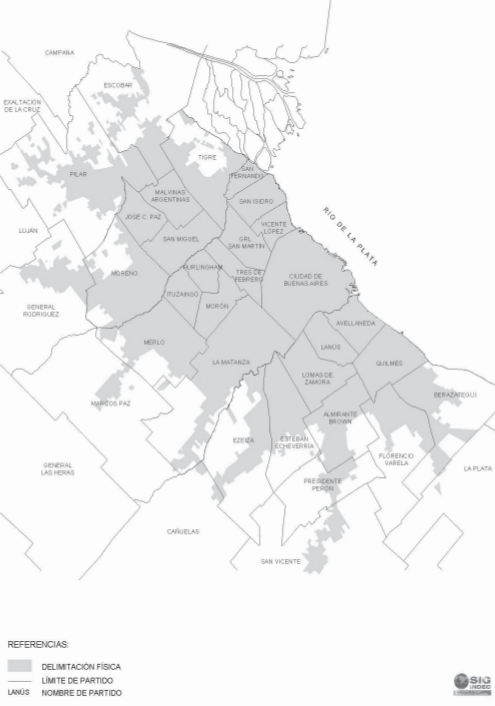
\includegraphics[scale = 0.4]{AGBA.png}
		\caption{Aglomeración Gran Buenos Aires - 2010. Fuente: INDEC}
	\end{center}
\end{figure}

Este criterio de delimitación se mueve con el tiempo y, por cierto, no respeta las delimitaciones administrativas de los partidos.  Estas peculiaridades y complicaciones que implica trabajar con unidades espaciales, serán consideradas con mayor precisión en el apartado metodológico. Tal cual la configuración que el Aglomerado Gran Buenos Aires asume en 2010, el mismo abarca la Ciudad de Buenos Aires y se extiende sobre el territorio de la Provincia de Buenos Aires, integrando la superficie total de 14 partidos, más la superficie parcial de otros 16 (esto sin contar una muy pequeña participación de los partidos de Cañuelas y La Plata).

La incidencia de la distribución del ingreso en el AGBA es de enorme relevancia en términos demográficos como económicos, dado que constituye la aglomeración urbana de mayor concentración de población del país \cite{indec2012}. A su vez, desde un punto de vista metodológico, presenta niveles sumamente heterogéneos en términos de estructura socio-espacial, por lo cual se puede considerar como una zona interesante para aplicar este tipo de análisis. 

En resumen, este trabajo pretende elaborar un método que permita aproximarse indirectamente a la distribución microespacial del ingreso de los hogares en las ciudades a partir del caso del AGBA. Entre los interrogantes que disparan este trabajo podemos enumerar los siguientes: 

\begin{itemize}
	\item ¿Qué fuentes de información disponible existen sobre el ingreso y las condiciones de vida de los hogares?
	\item ¿Qué relaciones existen entre las condiciones de vida de los hogares, según se miden en el Censo, y el ingreso de los mismos?
	\item ¿Es posible a partir de mediciones de esas características, ofrecer una aproximación al ingreso del hogar mediante un índice que contemple estas relaciones?
	\item ¿Cuál es la distribución espacial del ingreso de los hogares en la Aglomeración Gran Buenos Aires?
	\item ¿Qué es necesario realizar para expandir este análisis a otras regiones del país?
\end{itemize}

En este sentido, se procederá en primer lugar a explorar las fuentes (Censo 2010, EPH 2010 y EAHU 2010) e identificar variables comunes que den cuenta de las condiciones de vida de los hogares. Segundo, se procurará determinar las relaciones existentes entre las variables vinculadas a las condiciones de vida de los hogares y el ingreso, a partir de la EPH y EAHU. En tercer lugar, se intentará desarrollar un índice que permita estimar el ingreso de manera válida y significativa, en base a las variables de condiciones de vida asociadas a él, para a continuación aplicar el índice desarrollado al caso del AGBA y verificar sus potencialidades para dar cuenta de la heterogeneidad socioespacial del ingreso intraurbano. Por último, se analizarán potencialidades y limitaciones de la propuesta para su replicabilidad en otros contextos urbanos.


	\subsubsection{Justificación y viabilidad del proyecto}


Desde un punto de vista académico, contar con un análisis de una distribución espacial del ingreso puede resultar de mucha utilidad para futuras investigaciones. Por un lado, puede contribuir en tanto que insumo para realizar una estratificación territorial a la hora de seleccionar diseños muestrales en búsqueda de parámetros sobre variables correlacionadas al ingreso. También puede servir precisamente para constatar qué correlación existe en el espacio entre el ingreso y otras variables (oferta y demanda de servicios públicos, desempeño electoral de un partido político, etc.). A su vez, existen numerosas investigaciones que estudian la estructura socio espacial del espacio urbano a partir de estrategias multidimensionales (socioeconómicos, sociodemográficos, culturales) con diversas metodologías (\textit{linkage, factorial, cluster}) para las cuales un índice que pueda aproximarse al ingreso de los hogares a nivel microespacial puede ser muy valioso como insumo para uno de los componentes o factores. Finalmente, el componente geográfico de la distribución personal del ingreso puede reconducir a un análisis de tipo funcional, analizando especialmente el retorno al factor tierra en el espacio de la ciudad, es decir la renta urbana. 

Este tipo de análisis podría contribuir, en términos de políticas públicas, a fundamentar una política tributaria progresiva de los municipios. En este sentido la relevancia de un estudio de la distribución geográfica del ingreso, puede constituir un insumo relevante para el diseño, implementación y evaluación de políticas públicas en el ámbito de los gobiernos municipales, como también metropolitanos y/o regionales.

En relación a la viabilidad del proyecto, desde el punto de vista de la disponibilidad de los datos, se encuentra plenamente garantizada. El INDEC publica trimestralmente las microbases de la Encuesta Permanente de Hogares (EPH) y la cartografía de la Aglomeración Gran Buenos Aires. En relación a los datos censales, provee en su sitio de Internet de un lugar para correr scripts personalizados del lenguaje utilizado para procesamiento del censo (REDATAM) que permita construir indicadores e índices personalizados para diferentes subpoblaciones (personas, hogares), a la vez que permite producir resultados para cada radio censal como nivel máximo nivel de desagregación geográfica (o AREABREAK en términos del lenguaje de REDATAM). Por su lado, la Dirección General de Estadísticas y Censos del Gobierno de la Ciudad de Buenos Aires también ofrece las microbases de su encuesta de ingresos para el año de interés. Todos los insumos de datos, si bien en formatos de software privativos y licenciados, son plausibles de ser incorporados en los lenguajes de programación libres para estadística y análisis de datos R y Python para su procesamiento, análisis y posterior georeferenciación. El tesista domina estos lenguajes de programación debido a sus prácticas profesionales y académicas.
 
	\section{Antecedentes}

La lectura de los antecedentes académicos de este trabajo se encuentra orientada, fundamentalmente, por tres lineamientos de interrogación. En primer lugar, en la medida en que se procura investigar una forma de distribución del ingreso, la distribución espacial, es indispensable interiorizarse sobre las nociones teóricas de ingreso y aquellas vinculadas a la distribución del mismo. En segundo lugar, en virtud de esta forma específica de distribución, se hace necesario recorrer la literatura sobre el impacto que tiene el espacio y el territorio sobre aquella forma de distribución desigual de los ingresos. Más aún, como se ha de estudiar este fenómeno recortado a la Aglomeración Gran Buenos Aires (AGBA), es necesario profundizar en el rol del espacio urbano en general, y en el espacio urbano de dicha aglomeración en particular. Por último, se hace indispensable revistar el cuantioso y diverso set de instrumentos metodológicos que se han construido para medir este fenómeno, en búsqueda de sus fortalezas y debilidades, como así también procurar asimilar aquellos elementos que puedan ser asimilables en este trabajo, en la medida en que la información disponible así lo permita. Como toda búsqueda de tesoro, se hace necesario, obviamente, un tesoro, un mapa y una brújula.

	\subsection{El Tesoro: el ingreso y su distribución}
Para comenzar, a la hora de definir conceptualmente ingreso ha habido diversas corrientes con definiciones de diversos niveles de complejidad. La literatura más convencional en economía define ingreso como el flujo de recursos que recibe un agente económico correspondiente a las remuneraciones por la venta o arrendamiento de los factores productivos que posee. El ingreso puede ser pagado en bienes y servicios o en dinero. También se puede considerar ingreso todas transferencias que reciben los agentes económicos tales como subsidios, donaciones y otras. Sin embargo, existe otra corriente que ha estudiado el ingreso y su distribución, entre los que se encuentra Richard \citeA[p.~34]{titmuss}, que ofrece una definición más amplia y abarcativa: “todos los recibos que aumentan el mando de un individuo sobre el uso de los escasos recursos- de una sociedad en otras palabras, su acreencia neta de poder económico entre dos puntos de tiempo ... Por lo tanto, el ingreso es la suma algebraica de (1) el valor de mercado de los derechos ejercidos en el consumo, y (2) el cambio en el valor del stock de los derechos de propiedad entre el principio y el final del período en cuestión”. De este modo, se puede contemplar una dimensión meramente nominal y monetaria de ingreso, una dimensión real que incluya a su vez el poder de compra de ese ingreso monetario en relación a los precios de los bienes consumidos, como así también el cambio en el valor del stock de bienes que se poseen.

Los análisis de la distribución del ingreso en las ciencias sociales han puesto el foco principalmente en dos de sus dimensiones: la distribución funcional y la distribución personal \cite{bemis}. La primera refiere a la forma cómo el ingreso total se divide entre los distintos factores productivos como, por ejemplo, trabajo, capital y tierra a través del salario, la ganancia o la renta; la segunda da cuenta de cómo ese ingreso se distribuye entre los individuos u hogares de una determinada región geográfica, sin importar el origen funcional de ese ingreso, ya sea que los individuos deben ese ingreso a un salario, a ganancias o a rentas \cite{gasparini2001}. 

El origen del interés de la distribución del ingreso se encuentra en la economía política de David Ricardo \citeyear{ricardo} en su obra “Principios de Economía Política y Tributación” y fue seguido fuertemente por Karl Marx y el marxismo durante buena parte del siglo XX. Estas corrientes abordaron el tema desde la óptica funcional “El producto de la tierra –todo lo que se obtiene de su superficie mediante la aplicación aunada del trabajo, de la máquina y del capital- se reparte entre tres clases de la comunidad, a saber: el propietario de la tierra, el dueño del capital necesario para su cultivo y los trabajadores por cuya actividad se cultiva” \cite[p.~5]{ricardo}. Karl Marx tributó a esta corriente analizando la distribución entre capital y trabajo \cite{marx2004}, como así también ha provisto profusas conceptualizaciones sobre renta agraria como una forma de distribución funcional del ingreso que involucra particularmente al espacio \cite{marx2011}. 

Con el tiempo, el cambio de épocas y paradigmas en las ciencias sociales como así también cambios en el fenómeno estudiado en sí, el interés ha ido migrando de los análisis funcionales a los análisis centrados en la distribución personal. Por un lado los cambios en los paradigmas en economía al imponerse el esquema neoclásico o marginalista con su individualismo metodológico \cite{blaug}, por otro los cambios en la distribución del ingreso misma (ya que muchos individuos en la cima de la distribución personal deben su ingreso a salario por ser gerentes de empresas, CEOs y/o mano de obra altamente calificada, convirtiendo la distinción entre distribución funcional y personal en una mucho más difusa), han llevado a poner el acento en la distribución personal del ingreso \cite{altimir1986,gasparini2001}.

De especial interés para este trabajo, sin embargo, son los trabajos sobre distribución espacial o geográfica del ingreso. El abanico de trabajos sobre este tema varía de acuerdo a si toman al ingreso en su dimensión funcional o personal y de acuerdo a la escala de la unidad geográfica que toman como referencia. De este modo se encuentran trabajos que llevan adelante análisis de la distribución del ingreso personal en entre diversos países \cite{theil,milanovic2002,milanovic2005,davies} o entre diversas unidades subnacionales hacia el interior de un país de mayor o menor tamaño: regiones \cite{orsatti,artana}, provincias \cite{altimir1975} e incluso se puede analizar la distribución del ingreso hacia el interior de un aglomerado urbano \cite{gasparini2000,giayetto} . 

	\subsection{El Mapa: el papel del territorio en la distribución del ingreso}
	
	\subsubsection{Los primeros mapas: los estudios de la ecología urbana}

A la hora de analizar la distribución del ingreso hacia el interior de un espacio urbano, como la Aglomeración Gran Buenos Aires, es necesario tener en consideración los efectos que el espacio urbano tienen sobre esta distribución. De hecho, este ha sido un enorme aporte del urbanismo y la sociología urbana\cite{park,burgess1928,mckenzie,wirth,lefebvre,harvey,castells} al dar cuenta el modo en que la organización del espacio urbano y en especial del espacio residencial, se vuelve determinante en la distribución del ingreso (aunque también determinados por ésta) con importantes efectos que son necesarios tener en consideración. 

La primera referencia obligada a la hora de analizar la temática del espacio, la ciudad y la desigual distribución espacial del ingreso es la escuela de la Ecología Urbana de comienzos del siglo XX. Nace en la Universidad de la ciudad de Chicago, en EEUU, donde se comienza a desarrollar el paradigma de los modernos estudios urbanos, para el análisis del espacio, la ciudad y de la distribución de los diferentes grupos sociales en el mismo. Esta escuela se enmarcan los trabajos de Robert Park \citeyear{park}, Ernest Burgees \citeyear{burgess1928}, Roderick McKenzie \citeyear{mckenzie} y Louis Wirth \citeyear{wirth}.

Park se encuentra entre los primeros en establecer los fundamentos teóricos de esta escuela. Sienta las bases de la ecología humana, sobre los cuales se construye la escuela de la ecología urbana, y tiende a pensar la sociedad en analogía con las comunidades en las ciencias biológicas, y al espacio donde se desarrollan en términos de hábitat. Las dinámicas al interior de esa comunidad, y dentro del espacio que ocupan, son de cooperación en base a la diferenciación funcional producto de la división del trabajo. Eventualmente puede acaecer una crisis, caracterizada como ambiental, al surgir modificaciones de la relación entre la población y los recursos del hábitat para sostenerla. En este marco de crisis hay un aumento de la competición hasta el surgimiento de una nueva división del trabajo que se adapte a las nuevas condiciones de vida. En ese caso, el nivel de competición disminuye y se retorna a un nivel de cooperación que hace a la comunidad, y su hábitat, sustentable. En las sociedades humanas, existe una estructura que refuerza esta dinámica, que es la estructura institucional radicada en las costumbres y tradiciones. Este es el fundamento de la ecología urbana, basado en la ecología humana y en algunos elementos del estructural funcionalismo de Spencer \cite{park,betin,gottdiener}.

En relación a la temática de este trabajo, la escuela ecológica de Chicago desarrolló el concepto de predominio para abordar el tema de la desigual distribución espacial del ingreso. Lucha por la vida y conflicto constituyen las condiciones que presiden la relación entre los hombres y la relación hombre-ambiente, determinando cierta distribución territorial de los individuos y su especialización funcional (o “vocación” profesional). A través de procesos modelados de interacción (competición, conflicto, adaptación y asimilación), basados en un fuerte individualismo metodológico \cite{gottdiener}, Park \citeyear{park} explica la dinámica de los espacios urbanos. A su vez, plantea la idea de predominio como extensión de la competición y el proceso que describe la competición de los actores por situarse en la posición estratégica del territorio dado, lo que en el largo plazo determina las características generales de la comunidad urbana, asignando mayores valores del suelo a los espacios de predominio. A su vez plantea el concepto de sucesión para dar cuenta de los cambios en estas conformaciones: cuando una serie de acontecimientos que sobresalen de la comunidad cuando esta crece y se desarrolla, transformando sus características esenciales. Esto puede modificar los suelos y sus usos, convirtiendo un espacio estratégico en desventajoso o de industrial en residencial \cite[p.~78]{betin}. 
Sin embargo, no quedan del todo claras las causas de estos cambios, la gran mayoría queda a procesos exógenos, como el crecimiento demográfico, aumento de la densidad poblacional, una migración o una tendencia inercial al desarrollo tecnológico, que son los que a su vez deberían ser explicados \cite{betin,gottdiener}. “El vicio real del enfoque ecológico se encuentra en la indebida superposición entre factores explicativos y factores a explicar. El meollo de la investigación ecológica, según Park, reside en el estudio de las relaciones entre equilibrio biótico y equilibro social. La 'balanza biótica', definida por la relación recursos del hábitat/población, es también un producto social: los recursos del hábitat se determinan a través de las fuerzas productivas, del estado de la tecnología y de las relaciones de producción, de las cuales deberían ser factor explicativo” \cite[p.~84]{betin}.

Un discípulo de Park, Ernest Burguess \citeyear{burgess1928} elabora, en el marco del paradigma de la ecología urbana, una particular teoría del espacio con implicancias en la desigual distribución espacial del ingreso de acuerdo a los diferentes grupos sociales, a la que denominó Central Business District. En esta teoría el espacio de la ciudad se describe mediante una serie de círculos concéntricos que representan las fases sucesivas de expansión de la ciudad en relación a un distrito central. La distribución espacial del ingreso en esta teoría se encuentra dada por la ubicación de las viviendas en el esquema concéntrico. Las zonas de viviendas estarían en los círculos externos, el tercer y el cuarto, donde viven los obreros industriales y los sectores de más altos ingresos respectivamente. En esta teoría del espacio, los elementos de la distancia y el tiempo al lugar de trabajo son centrales. \cite{burgess1928,betin}. 

Por su lado Roderick McKenzie \citeyear{mckenzie} ofrece una mejor sistematización de la ecología urbana con una definición más precisa de la misma como “el estudio de las relaciones espaciales y temporales de los seres humanos bajo la influencia de las fuerzas selectivas, distributivas y apropiadas que actúan en el ambiente” \cite[p.~91]{betin}. Como se puede apreciar en la definición, la relación causal entre las relaciones socio-espaciales de los humanos y el ambiente queda fijada con un sentido unidireccional. En sus desarrollos, la dinámica de las ciudades y comunidades no difiere mucho del paradigma general de la ecología urbana: se pone el acento en el equilibrio entre dimensión y recursos, donde los cambios continúan siendo exógenos al sistema \cite{gottdiener}. 

Con respecto a la desigual distribución espacial del ingreso, McKenzie ofrece uno de los primeros desarrollos teóricos sobre los vecindarios: “'El efecto general de los continuos procesos de invasión y de ordenación subdivide la comunidad desarrollada en áreas bien definidas, cada una con su propia capacidad selectiva y su propia cultura'. Se trata de las áreas naturales, que también McKenzie define en relación al valor de los terrenos, creyendo que éste sea un índice suficiente para caracterizarlas respecto al centro ciudadano y para determinar su clasificación. Añade, sin embargo, algunas observaciones sobre la distribución de los habitantes en el tejido urbano en relación a caracteres como edad, sexo y estado civil, que confieren al concepto de área natural una connotación, menos vinculada a las rígidas referencias económicas” \cite[p.~92]{betin}.

La desigual distribución espacial del ingreso se sigue explicando en los mismos términos generales de la ecología urbana y su individualismo metodológico, como competencia por el espacio y los recursos, y a través del concepto de “invasión”. “Con la expansión cuantitativa de la ciudad se desarrolla, de modo particular, un proceso de diferenciación y de segregación social. Se desarrolla la competición para lograr posiciones más ventajosas, acompañada de una serie de 'invasiones'. La ciudad se convierte así en un escenario de amplias transformaciones que, sin embargo, no alcanzan nunca, para McKenzie, el grado de conflictos radicales y violentos o, de todos modos, relacionados con el choque de intereses divergentes entre grupos socialmente diferenciados” \cite[p.~93]{betin}.

Finalmente, a la hora de pensar el espacio desde la escuela ecologista McKenzie  problematiza el concepto al sostener que las distancias ecológicas y lineales no siempre coinciden, en la medida en que dos puntos pueden estar a distancias lineales diferentes (medidas en metros o kilómetros por ejemplo) mientras que pueden estar a distancias ecológicas equivalentes (medidas en unidades tiempo que se emplea en recorrerla \cite{betin,mckenzie}. De este modo el espacio es problematizado más allá de la mera expresión en unidades simples de distancia (aunque de algún modo el espacio sigue estando constreñido epistemológicamente a la neutral y ubicua fricción de la distancia tan propia de la física social) \cite{soja}. De este modo introduce, además de mayores complejizaciones en relación a la distancia y el espacio, otros elementos que influyen en la desigual distribución espacial del ingreso, tales como: la conformación de los hogares en términos de edad, sexo y estado civil de los integrantes.

Louis Wirth \citeyear{wirth} por su parte, en el ensayo \textit{Urbanism as a way of life} ofrece un análisis más elaborado de la cuestión urbana con una definición concreta de ciudad a partir de una serie de elementos que luego estructurarán su análisis, aunque de un modo donde el paradigma de la ecología humana, con sus limitaciones, seguirá primando. Define la ciudad como una “localización permanente, relativamente extensa y densa de individuos socialmente heterogéneos” \cite[p.~8]{wirth}. 

Wirth deduce de los caracteres propios del fenómeno urbano (heterogeneidad, tamaño y densidad) elementos sugestivos para la interpretación de los procesos sociales tanto a nivel estructural como a nivel del conocimiento y comportamiento humanos. Sostiene, en relación a la desigual distribución espacial del ingreso, que la heterogeneidad social de los habitantes de una ciudad es una función de la dimensión cuantitativa del agregado urbano, de su cantidad de habitantes y de su densidad. La heterogeneidad es el sustrato de la diferenciación social y la división del ambiente urbano en áreas naturales y la solidaridad de la comunidad se sustituye por los mecanismos de competición sociales y el control social formalizado en instituciones. A su vez arriesga que esto también impacta en la personalidad esquizoide del habitante urbano \cite{betin,castells}.

El espacio en Wirth “se convierte en un patrimonio raro que adquiere un valor económico distinto en las distintas partes de la ciudad. El espacio condiciona la organización social de la ciudad en el sentido de que influye, con su valor económico, en la distribución de los habitantes y en su comportamiento cotidiano, estableciendo en qué lugar deben residir, en qué lugar deben trabajar, etc. La falta de espacio obliga a frecuentes relaciones y ello facilita el conocimiento de las situaciones sociales y culturales contradictorias. La falta de espacio genera congestión en el movimiento de los habitantes. Surgen así tensiones y problemas que la ciudad moderna no logra solucionar fácilmente” \cite[p.~106]{betin}. Wirth constituye probablemente el autor más lúcido de la escuela ecologista, aunque sigue sufriendo los problemas de este paradigma. “Wirth, basando su definición sobre todo en número y densidad, se demuestra más ecólogo de lo que querría ser. En primer lugar, olvida que la variable heterogeneidad cultural es una variable independiente e importante para comprender la vida urbana con un enfoque sociológico y, en segundo lugar, que número y densidad son a su vez simples efectos de aquellos procesos económico-sociales y de aquellos valores que acompañan a la urbanización” \cite[p.~106]{betin}. A la hora de conceptualizar la desigual distribución espacial del ingreso ofrece un conjunto de variables (distancia al centro, especificación funcional-laboral, variables demográficas) que a su vez son las que deben ser explicadas. Para la ecología urbana el dominio de un grupo sobre otro, con el fin de apropiarse de los mejores espacios geográficos, según Robert Park \citeyear{park}, opera de igual forma, tanto en las poblaciones vegetales y animales, como en la de seres humanos. Este domino es el responsable de la configuración social del espacio urbano y mientras en las comunidades biológicas se produce por un poder natural, en las comunidades humanas se basa en el poder económico de los grupos poblacionales y en el valor del suelo”. Este, en resumen, es el gran problema de la ecología urbana. Para esta escuela el espacio, aún en su versión más compleja de McKenzie, no deja de ser una cuestión de influencia directa de un ambiente un habitat natural no problematizado sobre la acción humana y de distancias en relación a un centro. Su impacto en la dinámica social queda resumida a esta única dimensión. 

Al mismo tiempo, existe en los desarrollos de esta escuela un conjunto de prenociones sobre aspectos culturales de la vida en la ciudad con cierta rémora durkheimiana. Para la Escuela de Chicago, en torno al “vecindario” se juegan toda una serie de elementos durkheimianos como la preeminencia de relaciones primarias filiales y cooperativas de la comunidad versus las relaciones secundarias competitivas de la sociedad. Concibe a su vez cierta función estabilizadora en la propiedad de la vivienda vinculada a una noción de orden social y tradición rural o pre-urbana. Wirth tributa a esta la linea durkheimiana, al diagnosticar en el espacio urbano cierta anomia y formalización de lo social en instituciones en la ciudad. Al mismo tiempo estudia el impacto del ambiente urbano en la personalidad esquizoide, siguiendo a Simmel, ofreciendo como principal fundamento el mero aumento demográfico. Estas nociones ideológico-cultuales no constituyen un elemento de importancia para este trabajo por la temática que aborda, pero es necesario mencionarlas en la medida en que constituyen elementos teóricos en relación a la vivienda y a la desigual distribución espacial del ingreso, contra los cuales, la escuela de la teoría crítica elaborará los suyos propios. 

\subsubsection{El mapa del ingreso es el mapa del conflicto: la escuela crítica}

En contrapunto con esta escuela, surge la llamada “nueva sociología urbana” de manos de autores como Henri Lefebvre \citeyear{lefebvre}, Manuel Castells \citeyear{castells} y David Harvey \citeyear{harvey}, que pueden inscribirse en diferentes variantes del paradigma marxista o de la llamada teoría crítica. Esta escuela ofrece una conceptualización del espacio mucho más profunda y en estrecha relación con los procesos sociales más amplios, como así también aborda la dinámica de la desigual distribución espacial del ingreso de un modo superador de las nociones durkhemianas del ecologismo urbano. Los autores de la nueva sociología urbana ponen en relación el espacio urbano con la dinámica de producción, reproducción del modo de producción capitalista y el cambio social. El espacio se convierte en una dimensión de análisis fundamental para comprender los procesos sociales, entendiendo que éste es simultáneamente producto y productor de las relaciones y prácticas que lo atraviesan. Cada autor de esta corriente comparte este concepto dialéctico de espacio, aunque puede haber diferencias en torno al acento que se le pone a los marcos estructurales o a la acción de los actores, como así también al grado de “especificidad” o “autonomía” de lo urbano. De acuerdo a Soja (1989:77) en este debate en lugar de explorar con sensibilidad la mezcla de oposición, unidad y contradicción que define la dialéctica socio espacial, se puso más atención en la primacía causal: acción o estructura. Sin embargo, tienen en común la construcción de su andamiaje teórico como una crítica a las elaboraciones de la ecología urbana de la escuela de Chicago. 

El recorrido que trazan estos autores es, también, un recorrido en un sentido de mayor precisión. Lefebvre es el primero en introducir el espacio en el paradigma del materialismo dialéctico \cite{soja} como un factor a considerar, aunque, precisamente por ser el primero, pagando el precio de una generalidad propia de la filosofía. Castells por su lado, intenta ofrecer mayores precisiones en el marco de la teoría social tributaria del estructuralismo francés. Finalmente, Harvey ofrece elementos más concretos sobre el rol del espacio en los procesos sociales en general, y en la distribución del ingreso en particular. En lo sucesivo, se ofrecerán brevemente las nociones que los autores más importantes de esta escuela ofrecen sobre su concepto de espacio y de la desigual distribución del ingreso en el mismo. 

Henri Lefebvre tiene, según Edward Soja \citeyear{soja}, el privilegio de introducir en la teoría social del materialismo dialéctico el espacio como una dimensión fundamental para comenzar a considerar. Sus principales obras sobre el tema son El derecho a la ciudad, De lo rural a lo urbano, La revolución urbana y La producción del espacio, escritos entre 1968 y 1974. Lefebvre destaca un hecho que parece elemental pero que de algún modo parece haber sido obviado en teorizaciones pasadas sobre las relaciones sociales: que todas ellas suceden en algún lugar, en algún espacio. Toma la calle para dar cuenta de ello. "¿Qué es la calle?" Es el lugar (topo) del encuentro, sin el cual no caben otros posibles encuentros en lugares asignados a tal fin (cafés, teatros y salas diversas) (…). La calle y su espacio es el lugar donde un grupo (la propia ciudad) se manifiesta, se muestra, se apodera de los lugares y realiza un adecuado tiempo-espacio" \cite[p.~25]{lefebvre}. Destaca, en su análisis de las transformaciones de la ciudad de París en su tránsito hacia una ciudad comercial, sobre los vínculos entre la función, la forma y la estructura social en el espacio y su incidencia en este proceso \cite[p.~17]{lefebvre}. Esta relación del espacio con los procesos sociales queda explicitada en su naturaleza dialéctica: "la realidad urbana modifica las relaciones de producción, sin por otra parte, llegar a transformarlas. Se convierte en fuerza productiva, como ocurre con la ciencia. El espacio y la política del espacio 'expresan' las relaciones sociales al tiempo que inciden sobre ellas" \cite[p.~21]{lefebvre}. Frente al ecologismo urbano, sostiene que estos procesos urbanos se rigen por una dinámica de implosión-explosión en el crecimiento urbano, destacando los elementos de ruptura por sobre los de continuidad o evolución del ecologismo urbano \cite[p.~20]{lefebvre}. En relación a la desigual distribución espacial del ingreso Lefebvre continúa pensando la misma en términos de un centro y una periferia, de la dialéctica de la centralidad o de su negación.

Sin embargo, no ofrece demasiadas precisiones que puedan servir como guía teórica en investigaciones concretas. En su postura excesivamente crítica de lo que entiende por empirismo, plantea una definición de sociedad urbana como virtualidad: “sociedad urbana designa la tendencia, la orientación, la virtualidad, más bien que un hecho consumado" \cite[p.~8]{lefebvre}. Es el resultado de la urbanización completa de la sociedad y la realización de la industrialización. Sobre ese horizonte de futuro, la revolución urbana se define como el "conjunto de transformaciones que se producen en la sociedad contemporánea para marcar el paso desde el periodo en el que predominan los problemas de crecimiento y de industrialización (modelo, planificación, programación) a aquel otro en el que predominará ante todo la problemática urbana y donde la búsqueda de soluciones y modelos propios a la sociedad urbana pasará a un primer plano” \cite[p.~11]{lefebvre}.

Hacia 1972 Manuel Castells publica en Francia \textit{La Cuestión urbana}, su principal esfuerzo teórico en relación a esta temática. El mismo es igualmente crítico del ecologismo, aunque presenta diferencias teóricas con Lefebvre, poniendo mayor énfasis en el marco estructural de la acción de los actores, que en la acción en sí misma. 

En su crítica al ecologismo \citeA[p.~100]{castells} sostiene que “hay una variación concomitante entre la evolución de las formas ecológicas y de las formas culturales y sociales, sin que se pueda afirmar por ello que esta covariación sea sistemática ni, sobre todo, que las segundas sean producidas por las primeras”. Continúa: “por consiguiente, la simple descripción del proceso no nos informa sobre el complejo técnico-social (por ejemplo, sobre las fuerzas productivas y las relaciones de producción) que actúa en la transformación. Hay, por tanto, producción \textit{simultánea} y \textit{concomitante} de las formas sociales en sus diferentes dimensiones espacial y cultural. Se puede plantear el problema de su interacción, pero no partir de la proposición según la cual una de las formas produciría la otra. La tesis sobre la cultura urbana se ha desarrollado en una perspectiva empirista, en la que se ha tomado por fuente de producción social lo que era su marco” \cite[p.~104]{castells} .

En relación a Lefebvre sus desarrollos teóricos representan, para el sociólogo español, un avance frente a los conceptos del ecologismo urbano. En el marco del debate sobre el impacto de un \textit{habitat} urbano determinado sobre la vida social, el autor francés se propone estudiar más la práctica del \textit{habitar} que la ecología del \textit{habitat}. Sostiene que estos \textit{habitats} no se descubren como un río, sino que se les construye, se localizan los procesos que llevan a la estructuración o la \textit{desestructuración} de los grupos sociales en su \textit{habitar}. Es decir, que se integra a estos procesos el papel jugado por el 'marco espacial', lo que viene, por tanto, a negar el espacio únicamente como 'marco' para incorporarlo como elemento de una determinada práctica social \cite[p.~128]{castells}.

Castells propone superar esta “explicación por covariación” del determinismo ecológico, pero tampoco aferrarse al “espontaneísmo de la acción social y la dependencia del espacio respecto a él” que observa en Lefebvre, donde el espacio aparecería como pura ocasión de despliegue de las relaciones sociales que en él tienen lugar. Dice Castells citando a Lefebvre “El espacio 'es el resultado de una historia que debe concebirse como la obra de \textit{agentes} o \textit{actores} sociales, de \textit{sujetos} colectivos que operan en oleadas sucesivas... De sus interacciones, de sus estrategias, éxitos y fracasos, resultan las cualidades y propiedades del espacio urbano'. Si esta tesis significa que la sociedad hace el espacio, todo queda por explicitar en términos de determinación específica”. Castells sostiene que es correcto como postula Lefebvre “considerar a la ciudad como la proyección de la sociedad en el espacio”. Pero advierte “si bien es cierto que hay que superar el empirismo de la mera descripción geográfica, se corre el grave peligro de figurarse el espacio como una página en blanco sobre la que se inscribe la acción de los grupos y de las instituciones, sin encontrar otro obstáculo que la huella de las generaciones pasadas” \cite[p.~141]{castells}. 

Sostiene que este proceso debe concebirse más bien como un proceso dialéctico entre acción y estructura donde aquella acción social actúa sobre la misma estructura, no es tan solo puro vehículo de efectos estructurados, sino que produce otros nuevos. “Las combinaciones y transformaciones entre diferentes sistemas y elementos de la estructura se hacen por intermedio de prácticas sociales, o sea, de la acción de los hombres, determinada por su particular inserción en los diferentes lugares de la estructura así definida” \cite[p.~154]{castells}. A pesar de las afirmaciones de Soja, Castells no parece del todo insensible al carácter dialéctico del espacio. Soja ofrece una descripción para este carácter dialéctico del espacio, que es el atributo en común de esta escuela: "Si la espacialidad es a la vez resultado/encarnación y medio/presuposición de las relaciones sociales y la estructura social, su material de referencia, la vida social, debe ser vista como tanto dependiente y formativa en relación al espacio, un productor y un producto de la espacialidad" \cite[p.~129]{soja}.

Para Castells no hay teoría del espacio al margen de una teoría social general, explícita o implícita. Esta teoría social general que sostiene Castells es el estructuralismo marxista, con orígenes en Althousser y Poulantzas \cite[p.~84]{soja}. “No existe teoría específica del espacio, sino simplemente despliegue y especificación de la teoría de la estructura social, de modo que permita explicar las características de una forma social particular, el espacio, y de su articulación con otras formas y procesos históricamente dados (...). Se trata de superar la descripción de los mecanismos de interacción entre implantaciones y actividades para descubrir las leyes estructurales de la producción y del funcionamiento de las formas espaciales estudiadas, la oposición entre determinaciones natural y cultural del espacio debe superarse a partir de un análisis de la estructura social, considerada como proceso dialéctico de puesta en relación de dos tipos de elementos por medio de prácticas sociales determinadas por sus características históricas; la diferenciación de un espacio, la distinción entre las funciones y proceso que ponen en relación las diversas unidades carecen de significación si no se refieren a elementos teóricamente significativos, los cuales sitúan al espacio en el conjunto de la estructura social” \cite[p.~152]{castells}.

En lo que refiere a la desigual distribución espacial del ingreso, para el sociólogo español, la dinámica es diferente a la propuesta por el ecologismo y enfocada desde una óptica de estructura de clases o grupos sociales más que desde el individualismo metodológico. “Amparándose en el organicismo ecológico, se descuida un carácter fundamental del espacio humano, a saber, la contradictoria diferenciación de los grupos sociales. Pues la apropiación del espacio forma parte de un proceso de la lucha que afecta al conjunto del producto social, y esta lucha no es una mera competencia individual, sino que enfrenta a los grupos formados por la inserción diferencial de los individuos en los diversos componentes de la estructura social -mientras que el 'complejo ecológico presenta una distinción sin hacer ver una diferencia'” \cite[p.~148]{castells}. En este proceso dialéctico de producción social del espacio, a su vez, ocupa un lugar central apropiación diferencial del producto del trabajo (el ingreso): “el hombre se transforma y transforma su medio ambiente en la lucha por la vida y por la apropiación diferencial del producto de su trabajo”  \cite[p.~141]{castells}.

En 1973 el geógrafo David Harvey compendia en un libro denominado \textit{Justicia Social y la Ciudad } una serie de ensayos escritos en diversos momentos de su trayectoria académica, personal e ideológica. Sus primeros trabajos se enmarcan en el paradigma del urbanismo y la geografía clásicos, mientras que sus trabajos tardíos contribuyen a la tradición del materialismo dialéctico o marxismo. El nombre de los apartados en los que divide la obra, da cuenta de esto: los primeros 3 aparecen en el apartado Formulaciones Liberales y los segundos en Formulaciones Socialistas.  

Aún dentro del marco de lo que llama “formulaciones liberales”, Harvey realiza una enérgica defensa del rol del espacio en los procesos sociales y critica la perspectiva de la economía neoclásica y sus estudios regionalistas, que parecen vivir y trabajar en un mundo sin espacio. “El espacio era simplemente una variable en un marco conceptual ideado principalmente para el análisis económico aespacial. Cientistas y economistas regionales siguen mostrando una predilección para la comprensión de la economía y una incomprensión del espacio” \cite[p.~26]{harvey}. Al mismo tiempo, Harvey plantea los problemas que tiene el paradigma de la geometría euclidiana de la geografía tradicional para comprender los procesos sociales en su dimensión espacial, en la medida en que el espacio social no es isomorfo con el espacio físico.  \cite[p.~29]{harvey}.

Esta inexistencia de isomorfismo entre el espacio social y el espacio físico se sostiene en que diversos individuos y grupos sociales tienen diferentes valoraciones socio-culturales para un mismo espacio físico, que no pueden factorizarse simplemente en una representación euclidiana bidimensional del espacio. Esto asesta una herida en el trasfondo epistemológico del entendimiento del espacio del ecologismo urbano y de aquellas otras escuelas que han reducido el espacio a la mera fricción de la distancia. Es notable como en el análisis de la acción de los grupos sociales, en esta etapa del pensamiento de Harvey, se percibe la tensión entre el individualismo metodológico y la teoría de las clases sociales. “Existen comportamientos grupales diferenciados, algunos los cuales pueden ser explicables en términos de las características sociológicas del grupo (edad, ocupación, ingresos, etc.): y hay estilos distintivos de actividad que sugieren que lugares de la ciudad particularmente diferentes, tienen muy diferentes poderes de atracción. En estos casos, podría estar justificada una generalización a una geometría más continua; pero incluso aquí el trabajo de los geógrafos sugiere que el espacio está muy lejos de ser un simple espacio euclidiano. En este punto se involucra en la cuestión la pregunta por la naturaleza exacta de la superficie socioeconómica que nos ocupa y el problema de encontrar transformaciones adecuadas para permitir el análisis de los acontecimientos en la misma. En general, tenemos que concluir que el espacio social es complejo, no homogéneo, tal vez discontinuo, y, casi con total seguridad, diferente del espacio físico en el que el ingeniero y el planificador urbano suelen trabajar” \cite[p.~35]{harvey}.

Sin embargo, también se distancia, en una crítica en línea con la que hace Castells, del primer autor que retoma teóricamente el espacio dentro del materialismo dialéctico: Henri Lefebvre. En el prólogo a su libro \textit{Justicia Social y la Ciudad} (1993), Ira Katznelson sostiene que Harvey rechazaba la autonomía que el sociólogo francés atribuía a las relaciones espaciales. En cambio, Harvey no otorgaba al espacio una categoría ontológica en sí, sino más bien lo consideraba una dimensión social que moldea y es moldeada por la actividad humana. “Las formas espaciales son vistas no como objetos inanimados en el marco de ellos cuales los procesos sociales se despliegan, sino como elementos que contienen procesos sociales del mismo modo en que estos procesos sociales son espaciales” \cite[p.~3]{harvey}.

Al avanzar en términos positivos la definición de su concepto de espacio Harvey, ya en su etapa tardía de desarrollo intelectual, se adscribe honestamente a la tradición epistemológica del materialismo dialéctico, sosteniendo que la naturaleza del espacio se explica mejor por la práctica social que por una definición propia del apriorismo idealista kantiano. Con mayor nivel de precisión que Lefebvre y Castells, propone 3 conceptos para aprehender el espacio (absoluto, relativo y relacional) pero cuál es el más pertinente depende de la práctica social concreta y a la relación que establezca con ese espacio particular. El primero hace referencia a la acepción más tradicional como una existencia material independiente, el segundo concepto propone que se entienda el espacio como una relación entre los objetos que sólo existen porque existen objetos y se relacionan entre sí y finalmente el espacio relacional plantea el espacio considerado como algo contenido en los objetos en el mismo sentido en que un objeto puede decirse que existe sólo en la medida en que contiene dentro de sí mismo y representa las relaciones con otros objetos. 

Pero más allá de esta categorización sobre la representación del espacio, Harvey plantea el espacio se convierte en aquello que hacemos durante el proceso de análisis, más que previo a este. El espacio no se concibe con ninguna de estas categorías en sí de un modo a priori, sino que es una, dos o las tres de acuerdo a las circunstancias, planteando a la práctica humana como la clave de entendimiento de qué categoría corresponde utilizar para analizar el espacio. Antes que plantear la pregunta “¿qué es el espacio?” prefiere preguntarse cómo es que diferentes prácticas humanas crean y hacen uso de diferentes conceptualizaciones del espacio. Por ejemplo, la relación de propiedad  privada crea espacio absoluto donde opera un monopolio: el flujo de personas, bienes y servicios sucede en un espacio relativo ya que insume dinero y recursos para vencer la famosa fricción de la distancia (que en la teoría de Harvey es solo uno de los aspectos del espacio) y por último el espacio relacional se hace realidad en la renta o alquiler, que captura todas las fuerzas del mercado, la densidad demográfica y el poder de venta minorista que determinada parcela tiene por estar relacionada a otras. En sintonía con la epistemología del materialismo dialéctico, concluye que es la práctica social humana cotidiana la que crea esos conceptos \cite[p.~13]{harvey}.

A la hora de pensar la desigual distribución espacial del ingreso, Harvey articula a la definición amplia de ingreso propuesta por Titmuss (“dominio sobre los recursos escasos de la sociedad”) con su noción de espacio complejo y multidimensional no asimilable con el espacio físico bidimensional euclidiano, y en especial con su noción del espacio urbano y la ciudad. “Creo que es mucho más satisfactorio considerar a la ciudad como un sistema de recursos gigantesco, la mayor parte del cual es hecho por el hombre. Es también un sistema de recursos localizados en el sentido de que la mayor parte de los recursos del sistema de la ciudad de los que hacemos uso, no son ubicuos y su disponibilidad, por lo tanto, depende de la accesibilidad y la proximidad. El sistema urbano contiene así una distribución geográfica de los recursos creados de gran importancia económica, social, psicológica y simbólica (...) El ingreso real de un individuo puede ser cambiado al cambiar los recursos a su disposición. Este cambio puede ser provocado de diferentes maneras. La cantidad de un recurso libre, sin precio, (como el aire fresco y tranquilidad) puede ser alterada, el precio del recurso puede ser cambiado, también el costo de acceso al mismo. Hay, por supuesto, una conexión entre el valor de la tierra y la vivienda y el precio de los recursos, ya que los cambios en este se capitalizan en los cambios en aquel” \cite[p.~68]{harvey}. Existe, por lo tanto, una intensa relación entre el ingreso y la provisión de bienes y servicios por parte de la ciudad de diferentes modos. Esa se convierte su agenda de investigación, guiada por la pregunta sobre cómo cambios en la forma espacial de una ciudad y los cambios en los procesos sociales que operan en una ciudad redundan en cambios en el ingreso de un individuo. 

Pero para Harvey esta disponibilidad de recursos no es una mera función de distancia a la manera del ecologismo urbano, sino que lo inserta en su concepción diversa del espacio y en el no isomorfismo de espacio social y físico. Fundamentalmente, esa valoración socio-cultural es variable y heterogénea, cambiante de acuerdo a los individuos y grupos, por lo que no permite obtener una función de bienestar social homogénea. Al no existir el principio de utilidad cardinal del modelo económico neoclásico, y ser reemplazado por funciones de utilidad ordinales, no puede plasmarse en un set de coordenadas bidimensionales euclidianas. La proximidad a un bien o servicio, solo es positiva en tanto y en cuanto el ciudadano de una ciudad desee ser usuario del mismo y lo valore positivamente. Por brindar un ejemplo burdo, una idéntica cercanía, medida en distancia euclidiana en base a las coordenadas de 2 dimensiones X y Y, a una zona de recreación, bares y restaurantes puede ser un valor para un joven estudiante pero un disvalor para un adulto mayor jubilado. Para el primero incluso puede cuantificarse ese “ingreso” adicional que implica dicha proximidad como el ahorro en transporte a dicha zona. La cuantificación del disvalor es más compleja. El espacio social, entonces, varía en función de un set de variables multidimensional. Concluye que esto implica un serio problema para los estudios de análisis de la distribución del ingreso en el espacio urbano dado que dos individuos pueden tener dominio sobre una cantidad igual de recursos, pero si los valoran de manera diferentes, entonces tienen ingresos reales diferentes \cite[p.~81]{harvey}.

Harvey ofrece mayores precisiones sobre cómo este espacio social urbano influye concretamente sobre (y es influido por) la distribución del ingreso, produciendo el proceso de desigual distribución espacial del ingreso en la medida en que estos mecanismos de distribución del ingreso que ofrece el sistema urbano tal cual existe, son mayormente regresivos. “La redistribución del ingreso puede ser provocada por cambios en (1) la ubicación de los puestos de trabajo y la vivienda, (2) el valor de los derechos de propiedad, (3) el precio de los recursos para el consumidor. Estos cambios se ven afectados, a su vez, por las asignaciones de costos externos y beneficios para diferentes regiones en el sistema urbano y por los cambios en la accesibilidad y la proximidad. Los diferentes sectores una población buscan controlar estos mecanismos ocultos que gobiernan la redistribución a través del ejercicio del poder político. Es en la caja etiquetada como 'valores sociales y culturales' que todo el proceso se retroalimenta a sí mismo, ya que estos valores son a la vez causa y efecto (...). Pero también inherente a estos procesos sociales se encuentra la cuestión de la organización espacial. Los efectos de las externalidades son localizados, también lo son las oportunidades de empleo y de vivienda, beneficios de los recursos, enlaces de comunicación, etc. A su vez, el poder político se basa, en parte, de un modo localizado. Muchos de los mecanismos ocultos para redistribuir el ingreso dan fruto en el acto de ubicación” \cite[p.~86]{harvey}.

	\subsection{La Brújula: instrumentos para medir la distribución del ingreso}
	
Tal como se ha mencionado previamente, los análisis de la distribución del ingreso han sido muy diversos en la literatura de las ciencias sociales y esta variedad tiene su correlato en el instrumental metodológico escogido para la medición del fenómeno. Esta variedad responde, resumidamente, a tres cuestiones que se deben precisar a la hora de encarar un análisis de este tipo: en primer lugar, si ha de tomarse en cuenta el origen del ingreso (análisis funcional) o no (análisis personal); en segundo lugar la escala geográfica que recorta el análisis (análisis internacional, nacional, regional, provincial, urbano, microespacial) y finalmente la fuente de información a tomar (encuestas, censos, registros administrativos, etc.). Esta última es de especial interés en la medida en que la información disponible se convierte en la principal restricción del análisis. 

En este sentido, es necesario hacer explícitas las decisiones en torno a estos tres puntos, para avanzar en un recorte de la vasta bibliografía disponible y de este modo hacer foco en los trabajos que estén en línea con los objetivos de esta tesis. En relación al primer elemento (el tipo de ingreso), en este trabajo se ahondará en la distribución personal del ingreso, mientras que en el segundo (la escala geográfica) se procederá a analizar el mismo en una escala microespacial. Dadas estas restricciones, ahora es necesario avanzar sobre los antecedentes en torno a los trabajos basados en instrumentos metodológicos que tomen como fuentes los Censos Nacionales de Población, Hogares y Viviendas. Si bien las encuestas de empleo e ingresos registran la variable ingreso -lo que permite aplicar indicadores bien desarrollados como Gini, Theil, Atkinson, Línea de Pobreza, etc. \cite{worldbank,beccaria,altimir2002} sus muestras no ofrecen los niveles de desagregación geográficos deseados (la Encuesta Permanente de Hogares del INDEC ofrece resultados por aglomerado urbano y la Encuesta Anual de Hogares del Gobierno de la Ciudad por Comuna de la Ciudad Autónoma de Buenos Aires). 

\subsubsection{El índice de Necesidades Básicas Insatisfechas (NBI)}

En un primer momento, estos métodos de medición de distribución del ingreso con base en información censal se orientaron al fenómeno de la pobreza: su medición y localización para obtener mapas (imposible con fuentes muestrales). En el marco de esta búsqueda, en los años 70, a instancias de la Comisión Económica para América Latina (CEPAL) en Latinoamérica y en Argentina se comienza a aplicar la metodología de Necesidades Básicas Insatisfechas (NBI). Su principal objetivo es identificar hogares y personas que no alcanzan a satisfacer un conjunto de necesidades consideradas indispensables según niveles de bienestar aceptados como universales, utilizando la información censal. 
En Argentina, el NBI se presentó como una alternativa en el caso de fuentes que no indagaban ingresos de la población. Cabe recordar que el método de Línea de Pobreza solo se aplicaba al aglomerado Gran Buenos Aires \cite{indec1984}. En la Argentina el método NBI se aplicó por primera vez en 1984 con datos del censo 1980 y los resultados se publicaron en el volumen “La pobreza en Argentina” \cite{indec1984}. Luego se replicó la metodología con datos del censo 1991 en el estudio “Perfil de los hogares y de la población con Necesidades Básicas Insatisfechas (NBI)” \cite{indec1996}.
La metodología de NBI \cite{beccaria,indec2000a,indec2000b} consiste en definir un conjunto de indicadores que permiten identificar la satisfacción de las necesidades definidas como básicas, para posteriormente calificar como pobre al hogar que presente al menos una de las carencias seleccionadas. Los cinco indicadores que se utilizan para considerar pobre a un hogar son:

\begin{itemize}
	\item Hacinamiento: hogares con más de tres personas por cuarto.
	\item Vivienda: hogares que habitan en una vivienda de tipo inconveniente (pieza en inquilinato, vivienda precaria u “otro tipo”).
	\item Condiciones Sanitarias: hogares que no tuvieran ningún tipo de retrete.
	\item Asistencia Escolar: hogares con algún niño en edad escolar (6 a 12 años) que no asiste a la escuela.
	\item Capacidad de Subsistencia: con cuatro o más personas por miembro ocupado y, además, cuyo jefe tuviera baja educación (como máximo hasta 2do grado de escolaridad primaria).
\end{itemize}

Este índice, al calor de su aplicación, fue forjando críticas frente a sus limitaciones. Por un lado, algunos autores sostienen \cite{alvarez1997} que la probabilidad de cada hogar de ser identificado como pobre depende de su estructura demográfica. Por otro lado, para Boltvinik \citeyear{boltvinik1992} la incidencia de la pobreza depende de la cantidad de indicadores que se utilizan para definir la población con NBI. Pero en lo que refiere a los objetivos de este trabajo, la limitación fundamental radica en que a través del índice NBI no es posible distinguir entre grados de satisfacción de necesidades dado que la metodología incorpora indicadores que sólo captan situaciones extremas, considerándose a la pobreza como un fenómeno único y homogéneo, sólo susceptible de una clasificación dicotómica: pobre-no pobre \cite{indec1996,minujin}. 

En virtud de estas críticas y en el marco del censo 2001 el INDEC propuso una nueva metodología que, a partir del reconocimiento de la heterogeneidad de la pobreza, permita distinguir grados de intensidad de la privación y diferencias de composición al interior de los hogares identificados como pobres. En el documento de trabajo del INDEC \citeyear{indec2003c}  se define sucintamente pobreza como la exclusión debida a la carencia de recursos necesarios para acceder a las condiciones materiales de existencia típicas de una sociedad históricamente determinada. En el mismo documento, se sostiene que pueden diferenciarse algunas formas de pobreza más estructurales -o permanentes- que otras y esto se encuentra estrechamente relacionado con la naturaleza de los satisfactores de necesidades. Por una parte, se reconocen bienes cuya obtención demanda una provisión exitosa sostenida en el tiempo. La privación de estos satisfactores en el hogar suele exigir un gasto considerable para revertir el estado de carencia de los mismos \cite{katzman,boltvinik1990}. Por otra parte, hay bienes y servicios de consumo inmediato cuya provisión es renovada permanentemente o puede variar con mayor asiduidad. Los hogares que carecen de estos satisfactores no necesariamente han estado expuestos a una privación recurrente y pueden adquirir o recuperar, eventualmente, tales recursos con gastos de consumo corriente.

Estas definiciones establecen dos dimensiones sobre el fenómeno de la pobreza, que dan cuenta de la complejidad del mismo. De este modo se puede hablar, en un caso, de una privación en torno a la situación patrimonial, lo que implicaría una pobreza de orden más estructural y, en el otro, de privación en relación a los recursos corrientes, lo que implicaría una pobreza de orden más coyuntural.

Para el primer caso, la delimitación de aquello que se considera necesario estará referida directamente al núcleo irreductible de privación de cuya satisfacción depende la subsistencia. El sentido de ese “núcleo irreductible”, ha sido señalado por los especialistas en tanto conjunto de necesidades absolutas que trascienden las comparaciones entre países o personas y que remiten a la dignidad e igualdad esenciales del individuo considerado como ser humano dotado de capacidades de ser y funcionar integrado en una sociedad \cite{altimir1979,sen}.

Para el segundo, algunos especialistas han señalado esta tendencia en la que la noción de pobreza se ha ido ampliando desde la incapacidad de comprar bienes en el mercado (falta de ingreso), hasta la incorporación de aspectos tales como la estigmatización, la marginación social, el riesgo y la vulnerabilidad, y la falta de empoderamiento y de voz \cite{kanbur}.

Estas diferencias entre satisfactores fueron asociadas a distintas metodologías de medición de la pobreza. En el método de NBI, a la privación asociada a la falta de acceso a bienes y servicios tales como vivienda y educación, se la denomina genéricamente pobreza estructural y se relacionó con la visión tradicional del bolsón crítico de índole más crónica. Por su parte, la metodología de la Línea de Pobreza (LP) fue asociada a la pobreza más coyuntural dada por la insuficiencia de ingresos, más sensible a las fluctuaciones del ciclo económico \cite{katzman,boltvinik1990}. 

Este debate sobre la heterogeneidad de la pobreza y las limitaciones del índice NBI para registrar este fenómeno llevó a la construcción del Índice de Privación Material de los Hogares (IPMH), combinando encuestas y censos. La CEPAL \cite{bravo2000a,bravo2000b} ha avanzado en sugerencias de metodologías para avanzar en ese sentido. “Las estimaciones de ingreso, consumo y pobreza para áreas menores se han hecho posibles mediante la combinación de información de los censos de población y vivienda con encuestas de hogares y el desarrollo e implementación de modelos estadísticos apropiados. Se trata de aplicaciones útiles, que complementan y en ciertos aspectos significan mejoras respecto de los procedimientos tradicionales” \cite[p.~225]{bravo2000a}. En el marco de un seminario sobre población y pobreza convocado por el Instituto Nacional de Estadística e Informática (INEI) de Perú, se presentó una alternativa para estimar indirectamente los ingresos con datos censales. Jorge Bravo (2000), investigador de la Comisión Económica para América Latina y el Caribe (CELADE), presentó una metodología para obtener estimaciones indirectas de la distribución del ingreso de los hogares en un censo apoyándose en el análisis de una encuesta de hogares próxima en el tiempo. El modelo estadístico formulado consistía en una regresión lineal múltiple que estimaba el nivel de ingresos a partir de la cantidad de miembros económicamente activos, sus características individuales (como edad y años de escolaridad), las características de la vivienda y la zona de residencia. A lo largo de la década del 90 esta temática fue abordada por numerosos países. Ha habido aplicaciones de este tipo de métodos en Perú (con datos del censo de 1993/encuesta de 1995), Nicaragua (1995/93), Uruguay (1985/85), Ecuador (1990/94), República Dominicana (1993/96) y Paraguay (1992/97) \cite{bravo2000a,bravo2000b}.

 \subsubsection{El Índice de Privación Material de los Hogares (IPMH)}

En este marco el INDEC \citeyear{indec2000a,indec2000b,indec2003a,indec2003b,indec2003c,indec2003d} propuso una nueva metodología: un indicador de privación denominado Índice de Privación Material de los Hogares (IPMH). La principal característica de esta metodología es que, a partir del reconocimiento de la heterogeneidad de la pobreza, permite distinguir grados de intensidad de la privación y diferencias de composición al interior de los hogares identificados como pobres. El IPMH es una metodología de identificación y agregación de las diferentes situaciones de pobreza, según el tipo y la intensidad de las privaciones que afectan a los hogares. Procura ofrecer una aproximación a la privación percibiendo grados y situaciones diferenciales que reconocen el carácter estructural o coyuntural de las carencias. Para ello considera la condición de privación en relación a los recursos corrientes y a la situación patrimonial.

Se considera un espacio bidimensional donde se integran el logro de los hogares respecto de su patrimonio y respecto de los recursos para consumo corriente se pueden identificar distintos tipos de privación delimitados por el umbral de satisfacción de cada eje. En relación a la privación patrimonial se construye, en torno a la vivienda, un indicador de Condiciones Habitacionales combinando dos subdimensiones: una referida a la protección o abrigo del medio natural y de factores ambientales adversos, y otra relacionada al equipamiento mínimo para el desarrollo de ciertas funciones biológicas en condiciones saludables. Se consideró con privación en la dimensión habitacional a los hogares que carecen de inodoro con descarga de agua o que habitan en una vivienda con pisos o techos de materiales inadecuados.

En relación al segundo aspecto, el que respecta mayor interés para los objetivos de este trabajo, se construyó un indicador de Capacidad Económica (CAPECO) de los hogares, vinculado a la privación de recursos corrientes \cite{alvarez2002}. El mismo aproxima al nivel de ingresos del hogar, a partir de la relación existente entre los años de educación formal aprobados por los perceptores de ingresos y la cantidad total de miembros del hogar. Su significado es el de una tasa de dependencia ponderada por los años de educación de los miembros que forman parte de la mano de obra ocupada (o bien, que formaron parte de la misma y hoy reciben una pensión o jubilación). 

El indicador CAPECO se base en el supuesto de que la educación de las personas (específicamente los años de escolaridad aprobados en el sistema formal de enseñanza), asociada a otras características individuales tales como el sexo, la edad y el lugar de residencia, permiten estimar de forma bastante aproximada sus ingresos laborales. Esta relación es la base de la teoría del capital humano \cite{mincer,beckar,schultz1961,schultz1962} que calcula los retornos a la inversión en educación a partir de un modelo en el cual el logaritmo natural de los ingresos presentes es una función de los años de escolaridad aprobados por las personas. La forma inicial y más simple del modelo del capital humano expresa que las diferencias en los ingresos se explican a partir de las diferencias en la cantidad de años de escolaridad. El modelo se complejiza posteriormente para incluir variables como la edad, el sexo, la raza, la capacitación en el trabajo y otras formas de inversión en capital humano que se hacen en una etapa posterior a la escolar.

Una ventaja de CAPECO es ser aplicable a todos los hogares, independientemente de su composición y tamaño, pues considera la educación formal de todos los miembros perceptores. Asimismo, la formulación que se presenta posee una significativa relación con los ingresos del hogar \cite{indec2003a}. Los diseñadores del CAPECO establecieron como corte de privación para este indicador el valor que se encuentre por debajo de un umbral que se estableció de acuerdo al valor de la Línea de Pobreza correspondiente a Encuesta Permanente de Hogares de la (EPH, octubre 2001).

Cuando se combina las dos fuentes de información mencionadas (censo y encuesta), se pueden obtener estimaciones de ingreso y pobreza desagregadas geográficamente, que no se pueden conseguir sobre la base de una sola de las fuentes estadísticas. El método de estimación explota la disponibilidad de información común a los censos y las encuestas, referidas a características de la vivienda y de los hogares, de los individuos que las integran y de la zona donde residen.

\subsubsection{Los mapas del ingreso}

Estos y otros índices se han plasmado en el espacio urbano en numerosos trabajos que han intentado obtener mapas de desigualdad social urbana en escalas pequeñas.

En el campo internacional, entre los trabajos pioneros, se puede contar el trabajo de Charles Booth que en 1889 y 1891 publicó Life and Labour of the People in London, que contenía un mapa de la pobreza en los diferentes barrios de Londres aunque con una metodología no centrada en el ingreso y sin enarbolar una teoría especial sobre la relación entre el espacio, la ciudad y las prácticas sociales en general o de desigual distribución espacial del ingreso en particular. Durante el siglo XX en Estados Unidos tiene lugar el trabajo de Bell y Shevky (1955) que busca establecer áreas sociales homogéneas a partir de tres factores: segregación, urbanización y rango social o situación económica. Para esta última dimensión analizaron nivel de educación, nivel de empleo, clasificación laboral, grupo ocupacional, valor de la vivienda, valor del alquiler, hacinamiento, calefacción y refrigeración y otras variables. Luego compusieron un índice a partir de ocupación, grado escolar, precio de la vivienda. Metodológicamente trabajaron con datos básicos para cada área censal y su combinación posterior utilizando el método factorial dentro de los cuales el rango social era sólo una componente \cite{buzai2014,betin}.  En el trabajo de Castells se cita un trabajo de De Vise (\textit{Chicago's Widening Color Gap}) de 1967 sobre estratificación social en el área metropolitana de Chicago utilizando diversos indicadores para 10 municipios, siendo éstos la mínima unidad geográfica utilizada como desagregación. Para ello utilizaron las variables: proporción de empleo en diferentes categorías socio-profesionales, características demográficas y características de vivienda y renta media familiar (pero ésta calculada a su vez únicamente como la media del municipio, no para unidades menores).

Como trabajo pioneros en el análisis de las desigualdades sociales metropolitanas en Argentina sobre desigual distribución espacial del ingreso en espacios urbanos se puede citar el trabajo de Horacio Torres y Marta Schteingart \citeA{schteingart} en la década del 70. En este trabajo, y en otro no publicado, realizan una caracterización de sectores sociales en función de su nivel de ingreso, pero no ofrecen mayores elementos para determinar cómo fue realizada esa estimación. Torres posteriormente profundiza sus análisis en la dimensión micro-espacial \cite{torres1975,torres1978}. En estos trabajos pone el acento en variables como migración, régimen de tenencia y densidad, pero utiliza el coeficiente de personas por cuarto como principal indicador del nivel socioeconómico de un área y ofrece prueba empírica de la validez de dicha afirmación \cite{torres1975}. Intenta también utilizar variables educacionales y sanitarias para relacionarlas al hacinamiento. Este indicador se incorpora en otro trabajo \cite{torres1978} a un análisis de tipo cluster para computar un nivel socioeconómico multidimensional que incluye variables educativas y laborales. 

Con la aparición de los resultados del Censo de Población, Hogares y Vivienda de 2001 a nivel de radio censal, y el desarrollo contemporáneo de tecnologías SIG, a lo largo de la década del 2000, comienza a proliferar este tipo de análisis. En especial, se comienzan a desarrollar los denominados análisis microespaciales en la medida que la preocupación es visibilizar las diferencias sociales a nivel de pequeñas unidades espaciales. En este marco se realizan esfuerzos para la  actualización del mapa social de Horacio Torres a partir de indicadores univariados o multivariados de nivel socioeconómico \cite{thuiller,groisman,marcos2011,marcos2015,buzaimarcos2014}.

Es interesante destacar los trabajos más recientes de Buzai y Marcos \cite{buzaimarcos2014,marcos2015} por ser representativos de la metodología factorial de componentes principales, muy utilizada en los estudios microespaciales. La misma procura sintetizar información de las variables originales en un número mínimo e imprescindible de nuevas variables denominadas factores. Cada factor, en este sentido, representa la relación existente entre un conjunto de variables intercorrelacionadas, y explica el máximo de su varianza común, es decir, que los factores pueden interpretarse como las dimensiones subyacentes de un conjunto amplio de variables \cite{marcos2015}.  Se aproximan al componente económico de los hogares a través de numerosas variables censales: porcentaje de población de 25 o más años con nivel de instrucción terciario o universitario completo, porcentaje de población en viviendas censada en departamento, porcentaje de población en hogares con agua procedente de red pública y porcentaje de población en hogares con inodoro con descarga y desagüe a red pública. 

En general, estos trabajos precedentes han perseguido dos caminos: han procurado abordar el nivel socioeconómico definido de forma simple y sin tener en cuenta sus múltiples dimensiones, o han procurado abarcar esta multidimensionalidad vía la metodología factorial. No han partido de la búsqueda de un índice positivamente relacionado con el ingreso y validado estadísticamente (como CAPECO), para luego proceder a mapear los valores de dicho indica para las escalas geográficas deseadas.  Por lo tanto, queda por explicitar en estos trabajos la relación entre estas variables utilizadas y el ingreso: la variabilidad del ingreso explicada por estas variables, la magnitud de la relación de cada una de las variables y el ingreso y los márgenes de error, entre otros temas. Este trabajo pretende contribuir en ese sentido, ofreciendo respaldo empírico para los supuestos que asumen que determinados valores en esas variables implican determinado nivel de bienestar económico en esos hogares.

A modo de recapitulación a lo largo del capítulo se ha dado cuenta de la existencia de numerosos desarrollos que permiten fundamentar que el espacio tiene una fuerte incidencia en la distribución del ingreso (a la vez que el ingreso influye sobre la producción social del espacio) y que es una relación que merece ser analizada. Al mismo tiempo, se ha pasado revista a diversas metodologías para ofrecer una distribución del ingreso a nivel micro espacial para el análisis de esta temática tan importante, fundamentalmente el CAPECO, desarrollo por parte del INDEC en base a la metodología propuesta por CEPAL en el marco de los desarrollos sobre capital humano. Sin embargo, como \textit{agenda pendiente} emerge la imperiosa necesidad de una actualización de estos estudios frente a los nuevos datos del Censo Nacional de Población, Hogares y Vivienda 2010, no sólo para ofrecer un nuevo mapa imprescindible de la distribución del ingreso para el caso del AGBA, sino también para revisar la metodología y eventualmente proponer modificaciones allí donde sean necesarias. Este es el propósito de este trabajo. En sintonía con la clave de lectura propuesta aquí en los \textit{Antecedentes}, queda pendiente definir con mayor precisión teórica en el apartado siguiente: a) qué se entiende por ingreso en este trabajo (el Tesoro); b) qué tipo de relación se establece con el espacio urbano o qué se espera encontrar en un mapa de este ingreso (el Mapa); y, por último, c) los fundamentos teóricos del instrumento utilizado para medir el fenómeno (la Brújula).

	\section{Marco teórico}
	
	El presente trabajo tiene por objetivo elaborar un método que permita aproximarse a la distribución espacial del ingreso de los hogares hacia el interior de ámbitos geográficos de escalas reducidas, para luego aplicar este método en el AGBA con los datos del Censo Nacional de Población, Hogares y Viviendas de 2010. En este sentido, es indispensable ofrecer una definición del concepto \textit{ingreso } tal y como se lo entiende en el marco de este trabajo. Al mismo tiempo, y en la medida en que se analiza su distribución espacial y el papel que el espacio juega en ella, más allá de los análisis aespaciales de la economía neoclásica, es indispensable encarar una tarea similar con relación al concepto de \textit{espacio}. De manera similar a la economía neoclásica, la geografía moderna metodológicamente reducía el espacio a una entidad bidimensional euclidiana donde lo único que importaba era la neutral y ubicua fricción de la distancia, tan propia de la física social, y a la explicación por covariación del ecologismo urbano. Es necesario complejizar dicho análisis. Por último, se observó en los \textit{Antecedentes} que ha habido numerosas experiencias a la hora de ofrecer indicadores indirectos de la distribución del ingreso, inclusive trabajos sobre la distribución espacial del mismo. Se procederá a tomar en consideración esos aportes y recuperar los elementos metodológicos que contribuyan en mayor medida a los objetivos del trabajo.
	
	En conclusión, en este apartado se pretende retomar los debates abordados previamente para brindar mayores precisiones teórico-metodológicas sobre los conceptos fundamentales que estructuran este trabajo. Fundamentalmente, se trata de brindar definiciones sobre los tres ejes recorridos en los \textit{Antecedentes}: el ingreso (\ref{MT-Ingreso}), el espacio urbano (\ref{MT-Espacio}), la distribución espacial desigual de este ingreso en dicho espacio urbano (\ref{MT-DistribucionEsp}) y los elementos que teóricamente podrían conformar un índice que se aproxime a este fenómeno de distribución espacial desigual (\ref{MT-Fundamentos}).
	
	\subsection{El ingreso}\label{MT-Ingreso}
	
	David Harvey \citeyear{harvey} retoma en sus desarrollos teóricos sobre la justicia social y la ciudad el concepto de ingreso más amplio propuesto por Richard Titmuss \citeyear{titmuss}: “dominio sobre recursos”. En una economía de mercado, el ingreso es lo que garantiza el acceso, o dominio, sobre los recursos indispensables para la vida, sobre los bienes y servicios que garantizan la reproducción de los miembros de una sociedad en todas sus dimensiones, desde la más elemental (alimento, vestimenta, vivienda) hasta la más compleja (educación, salud, esparcimiento, etc.). En una economía de mercado, la mayoría de las transacciones se encuentra mediada por el dinero. De este modo, es el ingreso monetario el que permite el acceso a estos bienes y servicios, el comando sobre estos recursos. No obstante, esta no la vía excluyente, sino que existen también la autoproducción y el acceso a bienes llamados “libres”, que no tienen precio. Éstos dos últimos serán analizados más adelante, pero dada la centralidad del ingreso monetario en la economía de mercado, se comienza la exposición por este lugar.
	
	El ingreso monetario, constituye para la economía el retorno a los factores que contribuyen en la producción. En este sentido, el ingreso es la contracara de la producción de un bien o servicio. Todo lo que se produce involucra el trabajo y el capital que se invierte (haciendo abstracción de los insumos) que son retribuidos en el momento en el que el producto se vende en el mercado bajo la forma del salario y la ganancia respectivamente. Desde esta perspectiva, el ingreso monetario que todo sujeto recibe constituye un retorno puntual ya sea al trabajo realizado o a la inversión de capital comprometida, en el marco de un proceso de producción de un bien o servicio. Esto lleva a los análisis de la distribución del ingreso de tipo funcionales, frente a los del tipo personales, donde se \textbf{pone el foco en} la cantidad de dinero recibido y \textbf{hacienco abstracción de} su condición de retorno a tal o cual factor en particular \cite{lindemboim,monza,altimir1986,altimir2002,conade}.
	
	Se ha comentado brevemente en apartados anteriores, que esta distribución adolece de algunos inconvenientes a la luz de la complejización del proceso productivo \cite{altimir1986}. Pero en este apartado tiene sentido brindar otros elementos sobre la problemática de un análisis funcional, dado que es posible realizar un análisis de la distribución espacial del ingreso tanto en su dimensión personal como funcional. En especial considerando que el análisis funcional combinado con el espacial, sería un análisis interesante de realizar, fundamentalmente en lo relativo a un retorno muy ligado al espacio, y sin embargo también muy omitido por la teoría económica neoclásica: la renta. La renta constituye un retorno al dueño de un suelo que lo ofrece en alquiler para la realización de alguna actividad. Puede ser producción agropecuaria, producción industrial o servicios (oficinas, comercios, etc.). Su ligazón con la cuestión espacial es innegable y sería muy interesante de analizar. Sin embargo, excede los propósitos de este trabajo y hay numerosos inconvenientes teóricos (no siempre se separa al suelo como factor específico, en especial el suelo urbano, lo que hace que su retorno -la renta- se confunda con la ganancia o el interés, que son retornos a otros factores) y prácticos (los instrumentos de recolección de datos no recaban esa información y cuando lo hacen o replican esa confusión teórica, mezclando renta y ganancia-interés, o no lo recaban a nivel microespacial, la escala de interés de este trabajo) que dificultan en extremo esta tarea. La indagación en torno a la distribución funcional del ingreso  plasmada en el espacio urbano en la forma de renta urbana, queda para una agenda futura de investigación.
	
	Por lo tanto, en este trabajo se ha tomado la decisión de analizar el ingreso desde la perspectiva personal haciendo abstracción de la fuente funcional del mismo (ya sea ganancia, salario, renta u otros). En respaldo de esta decisión se puede agregar otro elemento de peso. La producción y la distribución de ese ingreso, comprendido ampliamente como “dominio sobre recursos”, es una actividad social que se encuentra estructurada más allá de la acción individual que implica un retorno a un factor productivo ofrecido en el mercado. El enfoque de la distribución personal permite incorporar al análisis algunos de esos condicionantes sociales que inciden, por un lado, en los elementos que generan un ingreso (y su magnitud) y, por el otro, en su distribución entre diferentes individuos, mucho de los cuales obtienen un ingreso sin haber ofrecido a cambio ni capital ni trabajo (ni tierra). Esta última situación es la realidad de numerosos perceptores de ingreso en el espacio urbano y quedaría al margen de un análisis funcional de la distribución del ingreso.
	
	\subsubsection{Ingreso monetario del hogar}
	
	\textit{El hogar como unidad doméstica}
	
	La economía neoclásica, partiendo del individualismo metodológico, elabora nociones del ingreso como retorno a un individuo que va al mercado a realizar ya sea un trabajo o un capital, omitiendo de algún la pertenencia de dicho individuo a agregados sociales más amplios (grupos, clases, sectores,etc.). Desde otras disciplinas de las ciencias sociales (sistémicas, estructuralistas, marxistas, etc), sea ha postulado el acento en la sobredeterminación de estas acciones individuales por estructuras o sistemas supraindividuales. Diversas perspectivas sociológicas han intentado ofrecer una síntesis teórica para el análisis de la acción social \cite{bourdieu1991,bourdieu2001} y éstas brindan mayor riqueza en términos de aportes a investigaciones empíricas concretas sobre estos temas \cite{soja}.
	
	En este sentido, existe una instancia \textit{meso}-social que constituye un pliegue entre estas dimensiones macro y micro de los procesos sociales (la producción y distribución del ingreso es uno de dichos procesos): la familia. La misma constituye una institución social que actúa como la mediación entre el entorno social macro y la acción individual micro, entre las decisiones del individuo y del contexto en el cual se formó. Es una instancia de mediación entre la estructura social y la acción social. En palabras atribuidas a Jean Paul Sartre, uno es lo que hace con lo que hicieron con uno. La familia es también una instancia de actualización de la estructura social: las generaciones pasadas formando a las futuras y ofreciéndoles el contexto para ese desarrollo. La familia en este sentido es un gozne entre las dimensiones que Wright Mills \citeyear{wrightmills} proponía como constitutiva de la imaginación sociológica: entre estructura, biografía e historia.
	
	Los trabajos de Susana Torrado también aportan un marco teórico sobre el concepto de familia. En el plano analítico, y particularmente desde la sociología, las familias interesan en tanto instancias mediadoras entre los fenómenos de nivel macrosocial (estructuras) y de nivel microsocial (comportamientos) \cite{torrado1998}. En la familia occidental contemporánea esta mediación se concretiza, a través de “diversos tipos de intercambios: de bienes sexuales; de bienes afectivos; de bienes económicos; de obligaciones jurídicas. Desde esa perspectiva, constituye un lugar de ejercicio del poder (entre cónyuges; de los padres con respecto a los hijos; del Estado con respecto al grupo), a la vez que un lugar de protección con respecto al poder (seguridad de un ámbito privado frente a la esfera pública). A través de estos intercambios, la familia es investida socialmente de múltiples misiones: a) asegurar la reproducción biológica de la población y de la fuerza de trabajo; b) regular la relación entre los sexos; c) regular la relación entre las generaciones; d) asegurar la reproducción de la estructura de clases sociales; e) contribuir a mantener el orden social” \cite[p.~15]{torrado2003}. Dicha concepción de la familia como institución social mediadora se repite en el trabajo de Elizabeth Jelin \citeyear{jelin}, quien le atribuye funciones similares a las enumeradas por Torrado, que van desde la convivencia y la sexualidad, hasta la producción y reproducción, tanto biológica (en su acepción más literal de reproducción de los miembros de una sociedad), como social (la reproducción más amplia entendida como el mantenimiento del sistema social, socialización temprana de niños y niñas) y cotidiana (en lo relativo al mantenimiento y subsistencia de los miembros de la familia) \cite[p.~46]{jelin}.
	
	\textit{El ingreso de los hogares}
	
	Como puede observarse, el rol de la familia es central en el dominio sobre los recursos indispensables para la vida, es decir, el ingreso (tal como es comprendido en la definición amplia de Titmuss). La organización social las actividades domésticas ligadas al mantenimiento y reproducción de la población (que incluyen la producción y el consumo cotidiano de alimentos y otros bienes y servicios de subsistencia, así como las actividades ligadas a la reposición generacional, es decir, tener hijos, cuidarlos y socializarlos, y atender a los ancianos) tienen un impacto en el ingreso. Por lo tanto, esta nodalidad de la familia en el conjunto de los procesos sociales, es válida también para el proceso de producción y distribución de la riqueza, del producto y el ingreso. Torrado \citeyear{torrado1981} sostiene, en \textit{“Sobre los conceptos 'Estrategias Familiares de Vida' y 'Proceso de Reproducción de la Fuerza de Trabajo': Notas teóricas-metodológicas”}, que el hogar es el colectivo donde los individuos resuelven la reproducción biológica y de sus condiciones materiales y no materiales de vida. Es en el hogar donde los miembros económicamente inactivos participan indirectamente de las relaciones de distribución de los bienes que son propias de la sociedad a la que pertenecen y el ámbito donde se delinean las estrategias familiares de vida. 
	
	Por su lado, Jelin \cite[p.~79]{jelin} también profundiza y desarrolla el lugar de la familia en la producción y distribución del ingreso, ya no solo el monetario (el trabajo remunerado y no remunerado de sus miembros, las transferencias de instituciones formales como el Estado, la ayuda de organizaciones sociales 'solidarias', los ahorros propios, rentas, inversiones, etc.), sino los otros dos tipos enumerados previamente (autoproducción y bienes libres).
	
	En este sentido, se puede sostener que la procedencia familiar de un individuo tiene un enorme impacto en su capacidad productiva y en su capacidad de hacerse con una porción de ese producto, es decir en la forma de accionar en el proceso social de la distribución del ingreso socialmente producido. Se podría comenzar por afirmar que un individuo con capital económico puede ponerlo en acción y obtener una ganancia a cambio como ingreso. Dicho capital es acumulable y transferible generacionalmente, precisamente a través de la familia en el marco del derecho normativo de los estados occidentales. Pero ese no es el único capital acumulable y transferible por la familia al individuo y a las futuras generaciones de dicha familia. Ciertas corrientes teóricas de la sociología han utilizado esa noción de “capital” \cite{bourdieu2001}, como un activo acumulable y disponible para poner en acción y sobre el cual se espera un retorno, para aplicarlo a las otras dimensiones de los procesos sociales: la cultural, las relativa a las relaciones sociales interpersonales y a la misma dimensión económica.
	
	La vertiente del “capital humano” \cite{mincer,beckar,schultz1961,schultz1962}, entiende que incluso al interior de los asalariados (cuyo ingreso corresponde funcionalmente al retorno del trabajo, no del capital) existen diferencias de capital económico, entendido este no como la acumulación previa de bienes y dinero, sino como la acumulación de conocimientos que ofrecen un retorno en la forma de mayor productividad en el trabajo y, por ende, mayor salario. De acuerdo al paradigma del capital humano, la educación se conceptualiza como una inversión que ofrece sus retornos, en primer lugar a garantizar participación en el mercado de trabajo y, en segundo lugar, ofreciendo al trabajador una mayor productividad de su trabajo por el cual obtendrá mayores salarios (presuponiendo que el salario es una función de la productividad del trabajo). El estudio panel de Sánchez Torres y Núñez Méndez \cite{sanchez} sobre decisiones del hogar en el espacio urbano en Colombia en relación a los retornos a la educación y la participación en la fuerza de trabajo, ofrecen evidencia empírica para este paradigma de que mayores años de escolaridad (en especial en relación a la educación superior y terciaria) y mayores niveles de participación en el mercado de trabajo se relacionan positivamente con mayores niveles de bienestar económico.
	
	Precisamente, estos capitales, cuyos saldos pueden ser tanto positivos como negativos en todas sus dimensiones, son acumulados y distribuidos por la familia. Jelin describe este momento de “acumulación originaria de capital” por parte de una familia desde el momento de su constitución como tal. También desarrolla como la pertenencia a una familia influye notoriamente en la probabilidad que un individuo tenga de apropiarse de un ingreso, entendido más allá del ingreso monetario para abarcar también el dominio sobre recursos como los bienes y servicios libres o gratuitos que provee un sistema urbano.  
	
	"En el momento de la unión, los miembros de la pareja incorporan al proyecto en común algunos recursos materiales (también compromisos futuros y deudas), cuya magnitud depende de la situación económica previa de cada uno, de la ayuda familiar (herencia y anticipos de herencia recibidos, compromisos económicos con otros familiares) y de la acumulación 'originaria' realizada por los novios en función del proyecto de unión (en los casos de matrimonio con todos sus rituales, éstos pueden incluir desde el ajuar de la novia y los regalos de casamiento hasta la vivienda propia). También traen a la unión su 'capital humano', es decir, las habilidades y capacidades (tanto como incapacidades) de cada uno/a, que se manifiestan en la disposición a trabajar y en el tiempo a ser dedicado a esas actividades. También se debe tener en cuenta el 'capital social' que consiste en la red de relaciones sociales, laborales, de parentesco y de amistad, a la que es posible acudir para obtener favores y servicios, (ya sea ayuda para conseguir trabajo o crédito o ayudas cotidianas en la cocina, la limpieza, etc.), y el 'capital cultural' que incluye -y/o excluye- los saberes e informaciones sobre la provisión de bienes y servicios requeridos para las diversas actividades a desarrollar, y que influirán en las maneras y actividades en que puedan desarrollarse, incluso las domésticas (por ejemplo, el conocimiento de los medios de transporte, el conocimiento de las normas de funcionamiento de las burocracias estatales o los servicios médicos, o -tan visible en el caso de migrantes rurales en la ciudad- el conocimiento de las reglas y de las formas de relacionarse con 'extraños' en la interacción urbana" \cite[p.~96]{jelin}.
	
	Se observa entonces que los individuos obtienen numerosos ingresos (monetarios o no) de diversas fuentes (laborales o no) en un influyente contexto familiar, a la vez que realiza numerosas tareas, hacia el interior de dicho contexto, de auto-producción y auto-consumo (vinculadas al ingreso no monetario). Estos ingresos individuales, sus fuentes y magnitudes, se relacionan en gran medida con los capitales (sociales, culturales, humanos) que la familia tiene a disposición para poner en juego. Estos elementos fundamentan la decisión de considerar el ingreso personal de los individuos teniendo en consideración el contexto familiar al que pertenecen a la hora de hacer un análisis de la distribución personal del ingreso.
	
	
	Antes de concluir, es interesante dar cuenta de un último elemento que sustenta la decisión En la medida en la que una familia dispone de capitales acumulados, los pone en juego, los circula y hereda, se podría argumentar que el abordar el proceso de producción y distribución del ingreso desde la perspectiva familiar permite, no solo dar cuenta de la distribución presente, sino también ofrecer elementos para pensar sus probables configuraciones futuras. El proceso de movilidad social (en cualquier sentido) no estaría del todo indeterminado, ni ofrece las mismas probabilidades a todos los individuos, en la medida en que no disponen de los mismos capitales. Prácticas como la herencia de capitales de todo tipo o la 'homogamia'(el matrimonio dentro de un mismo grupo o categoría social en términos de edad, clase social, identidad étnica, racial, religiosa y nacional \cite[p.~31]{jelin}) pueden ofrecer elementos para pensar ese proceso de condicionamiento a las probabilidades de la movilidad social.
	
	"La familia es una institución formadora de futuras generaciones. En este sentido, es una instancia mediadora entre la estructura social en un momento histórico dado y el futuro de dicha estructura social. A partir de esta función reproductora de la sociedad, la institución familiar tienda a transmitir y reforzar patrones de desigualdad existentes (...). Las propiedades y las riquezas se transmiten por herencia; los 'climas educacionales' tienen un efecto altamente significativo sobre los niveles educacionales de los niños, niñas y jóvenes.; las redes de relaciones sociales son acumuladas y transmitidas. O sea, existe una fuerte tendencia dirigida a que la institución familiar perpetúe los privilegios de quienes los tienen. En el otro extremo, cuando hay carencias y riesgos, la institución familiar tiende a reproducir el círculo vicioso de la pobreza, la marginalidad y la violencia" \cite[p.~197]{jelin}.
	
	Habiendo definido que se toma el ingreso personal, y habiendo establecido el papel de la familia como condicionante de dicho ingreso, es necesaria una ultima precisión teórica. El Censo Nacional de Población, Vivienda y Hogares (tal como su nombre lo indica), no releva datos sobre \textit{familias per se}, sino sobre \textit{viviendas} y \textit{hogares}. Por su lado, la Encuesta Permamente de Hogares releva datos sobre \textit{viviendas} y \textit{hogares}, pero al relevar ingreso (la variable en cuestión que se encuentra ausente en el Censo) lo hace bajo el nombre de \textit{ingreso familiar} (ya sea total o per cápita). Es por eso que es necesario ofrecer mayores precisiones en este sentido. 
	
	Habitualmente familia, vivienda y hogar se toman como sinónimos, sin embargo teórica y metodológicamente constituyen entidades diferentes, aunque cotidianamente existan límites difusos y solapamientos frecuentes. En las actividades de reproducción social ampliada que realiza una familia, la cercanía interpersonal es fundamental. Si bien pueden existir lazos familiares más allá de la copresencia en un mismo espacio (y durante la etapa de globalización y circulación internacional de flujos de personas, esta es una situación cada vez más cotidiana) hay una coincidencia significativa entre el grupo social que comparte la domesticidad familiar y el grupo conviviente. Si bien hay límites borrosos y situaciones ambiguas, es de esperar la coincidencia entre unidad residencial (vivienda), núcleo social doméstico (hogar) y núcleo familiar. 
	
	En conclusión, Luego de este análisis sobre el rol de estructurador social de la familia, en particular en torno a la producción y distribución del ingreso, es necesario ir precisando en términos teóricos el tipo de ingreso que se va a analizar en este trabajo. Se ha distinguido el ingreso monetario obtenido a través del mercado del ingreso no mercantil o no monetario. A su vez, este ultimo puede provenir de la autoproducción – autoconsumo o en el acceso a recursos a través de los bienes y servicios públicos, libres o gratuitos (de fuerte interconexión con las externalidades del sistema urbano).
	
	Dado que tanto el Censo como la EPH toman como unidades de análisis los hogares, en este trabajo se procederá del mismo modo. Se opta, en primer lugar, por trabajar con el ingreso monetario – mercantil y desde una perspectiva personal (haciendo abstracción de su fuente: trabajo, capital, renta). En segundo lugar, dado el rol central del núcleo social doméstico en el proceso de distribución del ingreso que se ha recorrido, no se toma el ingreso individual, sino que se considera al hogar como unidad. Por eso se toma el ingreso del hogar en so conjunto, sin considerar sus diversas fuentes relevadas en las encuestas.
	
	Por último y como se ha relatado, es evidente que un ingreso monetario de una magnitud dada, no implica un idéntico dominio sobre recursos si una hogar cuenta con escasos miembros dependientes o por el contrario éstos abundan \cite{buhmann}. De este modo, la conformación del hogar es central y a la vez da cuenta de un elemento fundamental: la etapa del ciclo vital que atraviesan sus miembros, si esas personas sean adultos mayores, adolescentes o niños. Tal como afirman Gaggero y Rossignolo "se han analizado diferentes alternativas para establecer la manera más apropiada de medición del bienestar de la sociedad. Las estimaciones iniciales otorgan la representación de la función al ingreso familiar; sucesivas reformulaciones plantean que el bienestar está mejor asociado al ingreso per cápita familiar, para concluirse en otros ajustes en el ingreso ajustado por adulto equivalente y economías de escala internas al hogar" \cite[p.~12]{gaggero} . En este sentido, y para concluir, en el marco de este trabajo se considera como ingreso el monto de ingreso per cápita del hogar.
	
	
	\subsubsection{Ingreso monetario y su vinculación con otros atributos de los hogares y las personas}\label{MT-Fundamentos}
	
	Serían los contenidos de tu sección 1.3.4, pero sin hacer alusión al espacio. Acá estás presentando conexiones teóricas presuntas entre ingreso monetario y otros atributos de los hogares y sus integrantes. Falta ponerle bastante más carne. ¿No hay nada citado en los trabajos de IPMH/ CAPECO que leíste? ¿O en los documentos originales de CEPAL? ¿No fundamentan teóricamente ellos la elección de variables?
	
	Este apartado pretende recuperar los elementos teóricamente vinculados al ingreso y a su distribución desigual en el espacio urbano para utilizarlos en la construcción de un índice capaz de dar cuenta del fenómeno a escalas microespaciales.
	
	Castells \citeyear{castells} menciona brevemente como dimensiones determinantes: la etapa en el ciclo de vida, la dimensión de la familia, el estatuto profesional, el nivel de instrucción, la pertenencia étnica y el ingreso como elementos a priori de interés teórico. Puntualmente ofrece tres elementos centrales a la hora de decidir sobre la vivienda por parte de una familia: la renta, la etapa en el ciclo de vida y la dimensión de la familia. “La 'elección' de una nueva vivienda toma en cuenta sobre todo la comodidad y la dimensión de la misma, así como su medio ambiente social. El emplazamiento y la accesibilidad con respecto al resto de la aglomeración apenas intervienen y tampoco el lugar de trabajo. El factor central en la decisión lo que hace que se tome o no, es el coste de la operación, que viene determinado por la renta, la etapa en el ciclo de vida y la dimensión de la familia”\cite[p.~215]{castells}.
	
	Jelin \citeyear{jelin} destaca los climas educacionales de los hogares, la inserción en el mercado laboral de sus integrantes, la etapa del ciclo vital de los mismos, y la composición del hogar, en términos de la cantidad de habitantes y la relación entre activos y dependientes.
	
	Como fundamento de la importancia de la educación como condicionante del ingreso, se puede recuperar los aportes del paradigma del capital humano \cite{mincer,beckar,schultz1961,schultz1962}. El mismo entendía los años de escolaridad de un individuo como una inversión que ofrece un retorno en forma de mayor productividad del trabajo del individuo y, entendiendo al salario como una función de la productividad, un mayor ingreso. A su vez, traza un vínculo entre mayores años de escolaridad en los miembros de una pareja que conforman una familia, con la composición del hogar en términos de cantidad de miembros y la proporción en el mismo de activos-dependientes.
	
	Por lo tanto, estas son algunas de las variables analizar que pueden tener impacto significativo en el nivel de bienestar del hogar, mejor representado de acuerdo a Gaggero \cite{gaggero} por ingreso per cápita familiar ajustado por adulto equivalente y economías de escala internas al hogar.
	
	Harvey también destaca la educación como una variable de enorme importancia a la hora de analizar la distribución espacial del ingreso, aunque vinculada no con el ingreso monetario familiar per cápita, del que se habla en el marco de este trabajo, sino en relación al ingreso indirecto que provee el sistema urbano que conforma parte de una agenda futura. Sostiene, de un modo algo similar a la noción de “capital cultural”, que estos años de escolaridad ofrecen también una mayor capacidad de entender el funcionamiento del sistema urbano. De este modo, los actores se encuentran más capacitados para sacar provecho del desarrollo desequilibrado y desigual del sistema urbano en términos de provisión de servicios, posicionándose mejor en él; y al mismo tiempo estos grupos tienen mayor afluencia en el sistema político para hacer que valer sus intereses sectoriales.
	
	“La cuestión principal aquí, por supuesto, es la velocidad con la que las diferentes partes de un sistema urbano pueden adaptarse a los cambios que ocurren dentro de ella ( ... ). Por lo tanto, es erróneo pensar en un ajuste en el sistema urbano como un procedimiento de proceso homogéneo a una velocidad uniforme ( ... ) Sería muy sorprendente si de hecho los grupos mejor educados y más ricos no habían tomado ventaja de este tiempo de retraso a una mayor sus propios intereses y mejorar sus propios ingresos. La asignación de recursos a continuación, se lleva a cabo como un ajuste a esta nueva distribución del ingreso y un proceso acumulativo de aumento de la desigualdad de la distribución del ingreso se pone en marcha. Ciertos grupos, en particular los que tienen recursos financieros y la educación, son capaces de adaptarse mucho más rápidamente a los cambios en el sistema urbano, y estas capacidades diferenciales para responder al cambio son una fuente importante en la generación de desigualdades”\cite[p.~56]{Harvey}.
	
	En conclusión, partiendo del análisis de estas variables es posible aproximarse al estudio de la distribución del ingreso de los hogares en el espacio urbano a escala microespacial. En los apartados que siguen, se plantea la hipótesis de trabajo, mayores precisiones metodológicas sobre las variables involucradas en el índice a construir y las tareas a realizar.
	
	
	
	
	
	
	\subsection{El espacio}\label{MT-Espacio}
	
	\subsubsection{El concepto de espacio}
	
	Se mencionó brevemente en los Antecedentes el recorrido teórico de la relación dialéctica de  las relaciones sociales y el espacio urbano en general y, en particular, cómo la distribución del ingreso se manifiesta en el proceso de la distribución desigual del ingreso en el espacio. Por lo tanto, dado que ya se ha definido qué se entiende en este trabajo por ingreso, y especificado a qué tipo de ingreso se hace referencia, para poder continuar en un análisis de la distribución espacial de ese ingreso en la Aglomeración Gran Buenos Aires, es necesario avanzar en mayores precisiones teóricas sobre dos aspectos centrales: por un lado el concepto de “espacio urbano” y por otro el de la distribución espacial desigual del ingreso y sus dinámicas.
	
	Tal como ha sido profusamente fundamentado por la nueva sociología urbana, para analizar cabalmente toda relación social, es indispensable incorporar el factor espacial, dar cuenta de cómo esta relación se plasma en el espacio. De otro modo, se renuncia a comprenderla en toda su complejidad. En este sentido, la apropiación del ingreso socialmente producido, relación social de lo más conspicua, no puede escapar a esta relación dialéctica con el espacio y debe ser incorporada en su análisis. En su derrotero teórico, la economía neoclásica no ha procurado muñir su andamiaje conceptual con una teorización del espacio y es, por lo tanto, insensible a los efectos que éste puede producir de modo específico en la propia distribución. Edward Soja sostiene que en la economía de Marshall, Pigou, y otros “la subordinación del espacio era tan grande que sus teóricos más influyentes orgullosamente produjeron nociones de una economía despolitizada que existían como si se estuviesen sólidamente compactadas en la cabeza de un alfiler, en un mundo de fantasía, prácticamente sin dimensiones espaciales” \cite[p.~32]{soja}. No se trata solamente de mencionar que la distribución del ingreso en una sociedad se plasma en el espacio, sino que a su vez la distribución espacial de las personas y hogares en una ciudad tiene impacto en cómo el ingreso socialmente producido se distribuye entre ellos. Para Raúl Castells la localización de polos sociales en la estratificación social, en los extremos tanto inferior como superior, va más allá de la “simple desigualdad de la distribución de las residencias en el espacio, a partir del momento en que la fusión de situaciones sociales y de las situaciones espaciales produce efectos pertinentes -o sea, de nuevo, específico de los datos espaciales- sobre las relaciones de clase, y de ese modo sobre el conjunto de la dinámica social” \cite[p.~213]{castells}.
	
	Es precisamente la escuela crítica, a la que Castells pertenece, la que contribuyó con la reconexión del concepto del espacio en tanto que forma de los procesos sociales, “un intento de explicar los resultados empíricos del desarrollo geográfico desigual (lo que los geógrafos inocentemente llamaron 'diferenciación espacial' o 'diferenciación aérea') a través de sus fuentes generativas en las estructuras organizativas, las prácticas y las relaciones que constituyen la vida social. Esta reconexión se afirmó, en principio, durante la década de 1950, cuando la llamada "revolución teórico-cuantitativa" surgió desde el corazón de la Geografía moderna, aunque, según Soja \citeyear{soja}, en una versión cada vez más técnica y matematizada de descripción geográfica. La misma, difería sólo superficialmente de la tradición neo-kantiana que ayudó para justificar el aislamiento de la geografía de la historia, las ciencias sociales, y el marxismo occidental. Se basa principalmente en la explicación de la física social, las ecologías estadísticas y estrechas referencias a la fricción ubicua de la distancia. “Pero después de todo lo realizado, los resultados continuaron explicando otros resultados en una regresión infinita de las geografías en las geografías, un conjunto de variables mapeables 'explicaban' otras a través de la "bondad" del ajuste” \cite[p.~51]{soja}.
	
	\subsubsection{El espacio urbano}
	
	Para superar este déficit teórico-metodológico en el análisis del espacio (urbano) y la distribución desigual del ingreso en el mismo, este trabajo toma los desarrollos de Castells que sostiene que no puede existir una teoría del espacio separada de una teoría de lo social en su conjunto. Consecuentemente con su marco de referencia, el estructuralismo althousseriano, todo análisis social debe abordarse a partir de la noción de estructura social, la cual se compone en tres instancias fundamentales: ideológica, político-institucional y económica (la fundamentalmente determinante). A la hora de abordar la “especificidad del espacio” en la teoría, sostiene que “la especificidad 'espacial' de la estructura social no es más que la expresión 'evidente' de una especificidad relativa a una de las instancias fundamentales de la estructura social o de sus relaciones” \cite[p.~277]{castells}. Pero advierte que “por especificidad no se trata de proponer un mundo aparte, sino de señalar la eficacia históricamente determinada de una cierta delimitación, con todas las articulaciones e interacciones a establecer entre tal subconjunto y la estructura social. Plantear la cuestión de la especificidad de un espacio, y en concreto del 'espacio urbano' equivale a pensar las relaciones entre los elementos de la estructura social, en el interior de una unidad definida en una de las instancias de la estructura social. Más concretamente, la delimitación de 'lo urbano' connota una unidad definida o bien en la instancia ideológica, o en la instancia político-jurídica o en la instancia económica” \cite[p.~277]{castells}.
	
	El foco en la primera de estas instancias, ideológica, ha llevado a los análisis en términos de la “cultura urbana” (como los de Wirth) que Castells sostiene no son los que pueden arrojar los frutos más ricos a la hora de la investigación. La político-institucional, a su vez, ha sido un criterio demarcatorio, definiendo una ciudad o municipio, pero argumenta que en el capitalismo avanzado hay un desacople entre fronteras políticas y la especificidad de su contenido social, ya que este se define fundamentalmente a nivel económico \cite[p.~278]{castells}. Ya hacia el interior de esta determinante instancia, los dos elementos fundamentales del proceso económico, los medios de producción y la fuerza de trabajo, la especificidad de los primeros lleva a los estudios regionales, al análisis de la disponibilidad de elementos técnicos para la producción, como así también de recursos naturales, elementos técnicos y productivos, etc. Los estudios urbanos, en cambio, deben poner el foco específicamente en la fuerza de trabajo. Este trabajo se nutre de estas definiciones sobre el espacio urbano y los procesos que lo estructuran. Fundamentalmente, en la medida en que se ha tomado la decisión de analizar la distribución personal del ingreso y por lo tanto se hace abstracción de los factores de producción (o medios de producción en la nomenclatura del marxismo althousseriano de Castels).
	
	De este modo se arriba a una definición del concepto de espacio urbano que se utilizará en el marco de este trabajo. “El espacio urbano se convierte así en el espacio definido por una cierta porción de la fuerza de trabajo, delimitada, a un tiempo, por un mercado de empleo y por una unidad (relativa) de su existencia cotidiana. Se puede pensar, por ejemplo, en la dificultad de establecer la unidad de una región urbana como elemento productivo (pues los flujos económicos forman una red continua), mientras que el mapa de migraciones alternantes sirve, por lo general, para delimitar un área urbana. 'Lo urbano', en tanto que connotación del proceso de reproducción de la fuerza de trabajo, y el 'espacio urbano', como contribuyendo a expresar las unidades articuladas de un proceso tal, son ambas nociones que nos permiten -a nuestro entender- el abordar teóricamente las cuestiones que acabamos de plantear” \cite[p.~279]{castells}. Enarbola finalmente una hipótesis de trabajo sobre el nodo central que estructura la producción del espacio urbano: “En las sociedades capitalistas avanzadas, el proceso que estructura el espacio es el referente a la reproducción simple y ampliada de la fuerza de trabajo; el conjunto de las prácticas llamadas urbanas connotan la articulación del proceso como el conjunto de la estructura social” \cite[p.~280]{castells}. 
	
	La centralidad del pensamiento de Castells sobre el espacio urbano para este trabajo radica precisamente en el énfasis que le otorga a la reproducción ampliada de la fuerza de trabajo, donde el ingreso constituye un elemento fundamental. “El espacio de consumo se referencia como el proceso espacial de reproducción de la fuerza de trabajo. Se pueden reagrupar bajo este título un conjunto de complejos procesos referidos a la reproducción simple y ampliada de la fuerza de trabajo en su relación al espacio: la habitación, espacios verdes, equipamientos y el aparato escolar y socio-cultural en el plano de la reproducción social e ideológica” \cite[p.~176]{castells}.
	
	En esta función de reproducción de los miembros de la sociedad, que Castells divide analíticamente en simple y ampliada, la familia, el núcleo hogareño, ocupa un lugar central. Por lo tanto, y siguiendo el criterio general de que toda relación social se plasma en el espacio, la encarnadura espacial de la familia (la vivienda) debe por lo tanto también ocupar un lugar de equivalente importancia.
	
	
	
	
	
	\subsubsection{El espacio residencial: hogares y viviendas}
	
	Entre estos procesos de reproducción de los miembros de la sociedad, y con ellos de la sociedad misma, el espacio residencial cobra especial importancia en la medida en que, a la hora de analizar el ingreso, se ha optado por elegir el ingreso per cápita de familiar. Una distribución espacial del ingreso, que incorpora la dimensión familiar como trascendental, necesariamente debe dar cuenta de la distribución en el espacio urbano de los espacios residenciales, de los lugares donde las familias deciden vivir, ya que esta es la decisión micro que los agentes sociales toman que, agregada, da cuenta del fenómeno macro que en este trabajo se intenta analizar.
	
	Para Castells este espacio residencial es fundamental dado que forma parte de la sub-instancia “Consumo” del determinante elemento económico de la estructura social, y la cual es especialmente dedicada a la reproducción de la fuerza de trabajo. El espacio residencial se estudia en la misma clave de análisis, entendiendo el espacio residencial como dialéctico, no producto de las voluntades de los compradores o inquilinos (como sostiene la vertiente culturalista de la ecología urbana), sino que la distribución de las personas en la ciudad, su decisión sobre donde habitar, como una acción social, parte de la relación dialéctica entre esta acción y la estructura que la enmarca (con sus efectos sobre la misma).
	
	En relación al espacio residencial sostiene, coherentemente con su teoría del espacio en general, que no se puede concebirlo como simple proyección de los valores de cada grupo. “En efecto, la sociedad no es pura expresión de culturas en sí, sino articulación más o menos contradictoria de intereses y por los tanto de agentes sociales, que no se dan nunca por sí mismos, sino siempre, y a la vez, en relación a algo distinto. Por lo demás, el espacio residencial no es una página en blanco donde los valores sociales vinieran a dejar su huella. Está, por un lado, históricamente constituido; por otro, articulado al conjunto de la estructura social, y no solamente la instancia ideológica” \cite[p.~136]{castells}.
	
	La vivienda, por lo tanto, es necesario entenderla como concepto teórico de una parte, en relación al lugar que ocupa en el conjunto del sistema económico, y de otra, como producto con las características específicas. Concerniente al primer punto, la vivienda es uno de los elementos esenciales de la reproducción de la fuerza de trabajo. “La vivienda es un bien diferenciado que presenta toda una gama de características en los concerniente a su calidad (equipamiento, confort, tipo de construcción, duración, etc.), su forma (individual, colectiva, objeto arquitectural, integración en el conjunto de habitaciones y en la región) y su estatuto institucional (sin título, en alquiler, en propiedad, en copropiedad, etc.) que determinan los roles, los niveles y las pertinencias simbólicas de sus ocupantes” \cite[p.~179]{castells} .
	
	Por otro lado, la vivienda entendida como producto del proceso productivo, puntualmente como producto de la industria de la construcción y de la inversión inmobiliaria, presente, en ciudades como la nuestra, el signo distintivo de la escasez, el déficit habitacional y condiciones inhabitables, que impactan notoriamente en los mecanismos de distribución espacial desigual del ingreso estudiados. “La vivienda depende, en su realización, de las características y objetivos de la industria de la construcción. En un primer nivel, quiere decir esto que, en ausencia de la intervención pública, la única demanda efectivamente considerada será la demanda solvente. Pues comparando las rentas de los matrimonios y los precios de los alquileres se deduce la dificultad de resolver la crisis únicamente por los mecanismos de mercado (…) No se trata, por lo tanto, únicamente de una estratificación en el consumo, al igual que existe para todos los bienes, en función de la estratificación social, sino, más directamente, de una no satisfacción de la demanda” \cite[p.~182]{castells}. En este marco de insuficiencia de vivienda, cuando el Estado no interviene, se produce “la invasión de terrenos libres por los que carecen de vivienda y la organización de un hábitat incontrolado regido por las normas culturales de sus habitantes, equipados de acuerdo a sus medios y que se desarrolla en lucha contra la represión policíaca, las amenazas jurídicas y a veces los atentados criminales de las sociedades inmobiliarias, derrotadas así en sus proyectos. Es este un fenómeno masivo en las grandes ciudades latinoamericanas” \cite[p.~203]{castells}.
	
	De este modo, los mecanismos que trabajan a la hora de la producción y distribución de la vivienda, son indispensables para analizar la distribución en el espacio urbano de los sectores de diversos ingresos. Castells ofrece algunos elementos que influyen en la calidad, el estatuto y la forma de la vivienda. “La vivienda es un mundo de signos, un mundo cargado de deseos y de frustraciones. La disposición de sus símbolos es altamente expresiva de la inserción social y de la evolución psicológica de sus habitantes. Sin embargo, es un marco pre-construido, producto de un proceso socio-económico general y su ocupación se hace según leyes de la distribución social. Así todas las encuestas sobre la movilidad residencial muestran la casi ausencia de 'elección' social: los movimientos se hacen en función de las necesidades de la familia, principalmente, según la dimensión y las posibilidades financieras, reguladas por el ritmo de la vida profesional. La cantidad, la calidad, el estatuto y la forma de la vivienda resultan de la conjunción de cuatro sistemas: el sistema de producción del bien duradero que representa; el sistema de distribución social de ese producto; el sistema de distribución social de los hombres (en función de su lugar en la producción y en la gestión); el sistema de correspondencia entre los dos sistemas de distribución” \cite[p.~202]{castells}.
	
	\subsection{Distribución espacial desigual del ingreso}\label{MT-DistribucionEsp}
	
	En este apartado se procurará dar cuenta de los elementos teóricos en torno a la distribución desigual del ingreso en el espacio urbano. En primer lugar, se puede destacar como uno de los elementos más influyentes la localización de los sujetos, agrupados en familias, en ese espacio urbano. Estamos hablando de la distribución de las familias y del espacio residencial en el entramado urbano. Ésta, a su vez, se encuentra relacionada (dialécticamente, en tanto que relación espacial) con la provisión de equipamientos y servicios que, como sostiene Harvey \citeyear{harvey}, todo sistema urbano provee.
	
	Castells resume esta relación entre la distribución de las familias y sus características, el espacio residencial y la provisión de servicios y equipamientos. “La distribución de las residencias en el espacio produce su diferenciación social y específica del paisaje urbano, ya que las características de las viviendas y de su población fundamentan el tipo y el nivel de los equipamientos y de las consiguientes funciones” \cite[p.~203]{castells}.
	
	Según Castells el proceso de distribución de las viviendas depende fundamentalmente de lo que él denomina “capacidades sociales de los sujetos”: el ingreso, el estatuto profesional, el nivel de instrucción, la pertenencia étnica y la fase del ciclo de vida. Toma en consideración de este modo, lo que en otras conceptualizaciones retomadas en este trabajo se consideran los capitales sociales, culturales y económicos de los sujetos, y su agregación en el núcleo hogareño familiar.
	
	“La distribución de los lugares de residencia sigue las leyes generales de la distribución de los productos y, por tanto, produce reagrupaciones en función de la capacidad social de los sujetos, o sea, en el sistema capitalista, en función de sus rentas, de su estatuto profesional, del nivel de instrucción, de la pertenencia étnica, de la fase del ciclo de vida, etc. Se hablará, por tanto, de una estratificación urbana correspondiente a un sistema de estratificación social (o sistema de distribución de los productos entre los individuos y los grupos), y en el caso en que la distancia social tiene una fuerte expresión espacial, de segregación urbana. En un primer sentido, se entenderá por segregación urbana la tendencia a la organización del espacio en zonas de fuerte homogeneidad social interna y de fuerte disparidad social entre ellas, entendiéndose esta disparidad no sólo en términos de diferencias, sino de jerarquía” \cite[p.~205]{castells}.
	
	Estas características del núcleo hogareño, le permiten acceder a espacios urbanos diferenciados por esa provisión de servicios y equipamientos. A su vez, dialécticamente, esta distribución diferencial de las familias y del espacio residencial, vuelve a influir sobre esa provisión que el sistema urbano genera. De este modo, el interés por problematizar los espacios residenciales de las áreas urbanas se basa en entender que la vivienda, tal como sostiene Sala \citeyear{sala}, no es sólo una unidad particular sino “parte de un colectivo que permite una mejor circulación de sus habitantes hacia los centros de la actividad laboral, el acceso a los servicios educativos y de salud y el desarrollo de actividades en el interior de las redes sociales”.
	
	Esta relación dialéctica entre espacio residencial y provisión de equipamientos y servicios, sucede en un espacio urbano fragmentado y desigual. El acceso a esos espacios privilegiados, en el marco de una economía de mercado, conlleva un costo. Es por ello que la localización de las familias en el espacio urbano guarda una relación con sus características (capitales de los que dispone), que a su vez se relacionan con el ingreso del que disponen. Una vez localizada una familia, en función de su ingreso, el mismo  vuelve a ser afectado por el espacio urbano.
	
	“Creo que es mucho más satisfactorio considerar a la ciudad como un sistema de recursos gigantesco, la mayor parte del cual es hecho por el hombre. Es también un sistema de recursos localizados en el sentido de que la mayor parte de los recursos del sistema de la ciudad de los que hacemos uso, no son ubicuos y su disponibilidad, por lo tanto, depende de la accesibilidad y la proximidad. El sistema urbano contiene así una distribución geográfica de los recursos creados de gran importancia económica, social, psicológica y simbólica (...) El ingreso real de un individuo puede ser cambiado al cambiar los recursos a su disposición. Este cambio puede ser provocado de diferentes maneras. La cantidad de un recurso libre, sin precio, (como el aire fresco y tranquilidad) puede ser alterada, el precio del recurso puede ser cambiado, también el costo de acceso al mismo. Hay, por supuesto, una conexión entre el valor de la tierra y la vivienda y el precio de los recursos, ya que los cambios en este se capitalizan en los cambios en aquel”\cite[p.~68]{harvey}.
	
	Harvey ofrece mayores precisiones sobre cómo este espacio social urbano influye concretamente sobre (y es influido por) la distribución del ingreso, produciendo el proceso de desigual distribución espacial del ingreso en la medida en que los mecanismos de distribución del ingreso que ofrece el sistema urbano tal cual existe, son mayormente regresivos. “La redistribución del ingreso puede ser provocada por cambios en (1) la ubicación de los puestos de trabajo y la vivienda, (2) el valor de los derechos de propiedad, (3) el precio de los recursos para el consumidor. Estos cambios se ven afectados, a su vez, por las asignaciones de costos externos y beneficios para diferentes regiones en el sistema urbano y por los cambios en la accesibilidad y la proximidad. Los diferentes sectores una población buscan controlar estos mecanismos ocultos que gobiernan la redistribución a través del ejercicio del poder político. Es en la caja etiquetada como 'valores sociales y culturales' que todo el proceso se retroalimenta a sí mismo, ya que estos valores son a la vez causa y efecto (...). Pero también inherente a estos procesos sociales se encuentra la cuestión de la organización espacial. Los efectos de las externalidades son localizados, también lo son las oportunidades de empleo y de vivienda, beneficios de los recursos, enlaces de comunicación, etc. A su vez, el poder político se basa, en parte, de un modo localizado. Muchos de los mecanismos ocultos para redistribuir el ingreso dan fruto en el acto de ubicación” \cite[p.~86]{harvey}. Otros estudios han destacado esta dimensión de la localización de la vivienda en relación con todo el conjunto de servicios proporcionados por una estructura urbana que conlleva la accesibilidad relativa a los beneficios sociales y económicos de otras unidades y actividades urbanas, entendidas como una serie de externalidades —acceso a servicios públicos, transporte, educación, cercanía a la fuente de trabajo, etc.— en función de su ubicación en el espacio 	\cite{yujnovsky,oszlak}.
	
	Estos mecanismos ocultos, que vuelven a reforzar la tendencia a la distribución desigual de los ingresos, constituyen un área de notable interés en una agenda futura de trabajo, de la cual un primer análisis exploratorio de la distribución espacial desigual del ingreso en la Aglomeración Gran Buenos Aires, constituye un primer y necesario escalón.
	
	Antes de concluir el apartado, es interesante observar cómo esta relación espacial dialéctica se encuentra medida por la institución familiar. "Las actividades domésticas ligadas al consumo consisten en transformar los bienes producidos y comercializados en el mercado. Para su realización, es fundamental la provisión de bienes y servicios colectivos -agua corriente, electricidad, drenajes, transportes, comunicaciones- así como servicios de educación y salud. Esta provisión de servicios -cuáles, para quiénes, a qué costo- constituye un frente de lucha donde históricamente se fueron planteando los temas de la incorporación de sectores sociales marginados a los derechos de la ciudadanía social. En realidad, la responsabilidad en la provisión de diversos servicios es de tal importancia que se ha convertido en una dimensión definitoria de los diversos modelos de Estado (...) La historia de las transformaciones del papel social del Estado puede ser leída como la historia de las luchas por la ampliación de derechos sociales, por la expansión de las políticas distributivas y por la extensión de los bienes y servicios colectivos, todas ellas ligadas a las actividades cotidianas de cuidado y reproducción" \cite[p.~91]{jelin}. De este modo, la provisión de servicios y equipamientos por parte del entramado urbano, y el nivel de mercantilización de los mismos, influye en las tareas domésticas del núcleo familiar, con fuerte peso en las mujeres de hogar, y en el ingreso disponible del mismo. "En realidad, la variación en la carga de la labor doméstica para las mujeres-madres, además de estar ligada obviamente a la composición del hogar, no depende tanto de la distribución de tareas y responsabilidades dentro del hogar (entre los miembros), sino fundamentalmente del acceso diferencial de las mujeres a servicios fuera del hogar (...) En la medida en que la oferta de servicios de este tipo esté centrada más que nada en los mecanismos de mercado, por los cuales hay que pagar, la variación fundamental se producirá entre clases sociales y niveles de ingreso" \cite[p.~97]{jelin}.
